\pdfminorversion=4
\documentclass[aspectratio=169]{beamer}

\mode<presentation>
{
  \usetheme{default}
  \usecolortheme{default}
  \usefonttheme{default}
  \setbeamertemplate{navigation symbols}{}
  \setbeamertemplate{caption}[numbered]
  \setbeamertemplate{footline}[frame number]  % or "page number"
  \setbeamercolor{frametitle}{fg=white}
  \setbeamercolor{footline}{fg=black}
}

\usepackage[english]{babel}
\usepackage[utf8x]{inputenc}
\usepackage{tikz}
\usepackage{courier}
\usepackage{array}
\usepackage{bold-extra}
\usepackage{minted}
\usepackage[thicklines]{cancel}
\usepackage{fancyvrb}

\xdefinecolor{dianablue}{rgb}{0.18,0.24,0.31}
\xdefinecolor{darkblue}{rgb}{0.1,0.1,0.7}
\xdefinecolor{darkgreen}{rgb}{0,0.5,0}
\xdefinecolor{darkgrey}{rgb}{0.35,0.35,0.35}
\xdefinecolor{darkorange}{rgb}{0.8,0.5,0}
\xdefinecolor{darkred}{rgb}{0.7,0,0}
\definecolor{darkgreen}{rgb}{0,0.6,0}
\definecolor{mauve}{rgb}{0.58,0,0.82}

\title[2019-09-14-awkward-strangeloop]{Jagged, ragged, awkward arrays}
\author{Jim Pivarski}
\institute{Princeton University -- IRIS-HEP}
\date{September 14, 2019}

\usetikzlibrary{shapes.callouts}

\begin{document}

\logo{\pgfputat{\pgfxy(0.11, 7.4)}{\pgfbox[right,base]{\tikz{\filldraw[fill=dianablue, draw=none] (0 cm, 0 cm) rectangle (50 cm, 1 cm);}\mbox{\hspace{-8 cm}
\includegraphics[height=1 cm]{princeton-logo-long.png}\hspace{0.1 cm}\raisebox{0.1 cm}{
\includegraphics[height=0.8 cm]{iris-hep-logo-long.png}}\hspace{0.1 cm}}}}}

\begin{frame}
  \titlepage
\end{frame}

\logo{\pgfputat{\pgfxy(0.11, 7.4)}{\pgfbox[right,base]{\tikz{\filldraw[fill=dianablue, draw=none] (0 cm, 0 cm) rectangle (50 cm, 1 cm);}\mbox{\hspace{-8 cm}
\includegraphics[height=1 cm]{princeton-logo.png}\hspace{0.1 cm}\raisebox{0.1 cm}{
\includegraphics[height=0.8 cm]{iris-hep-logo.png}}\hspace{0.1 cm}}}}}

% Uncomment these lines for an automatically generated outline.
%\begin{frame}{Outline}
%  \tableofcontents
%\end{frame}

% START START START START START START START START START START START START START

\begin{frame}{Motivation: particle physics analysis}
\Large
\vspace{0.35 cm}
\begin{columns}
\column{0.48\linewidth}
\only<1>{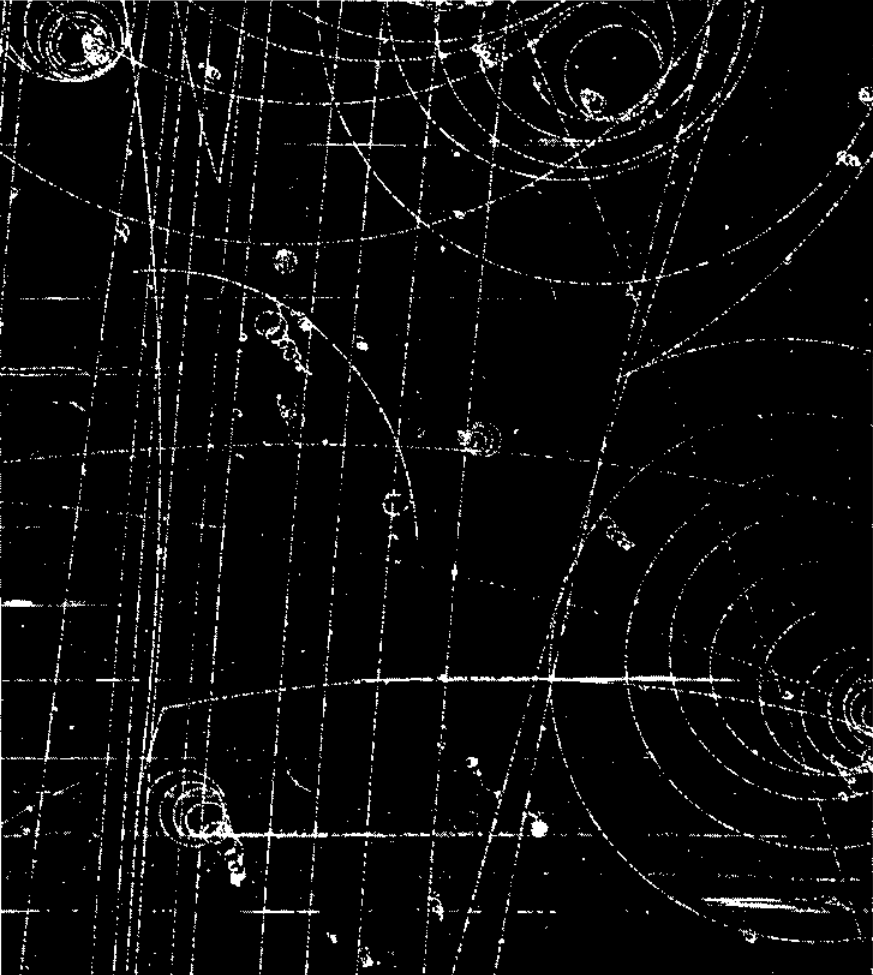
\includegraphics[width=\linewidth]{omega-minus-1.png}}\only<2->{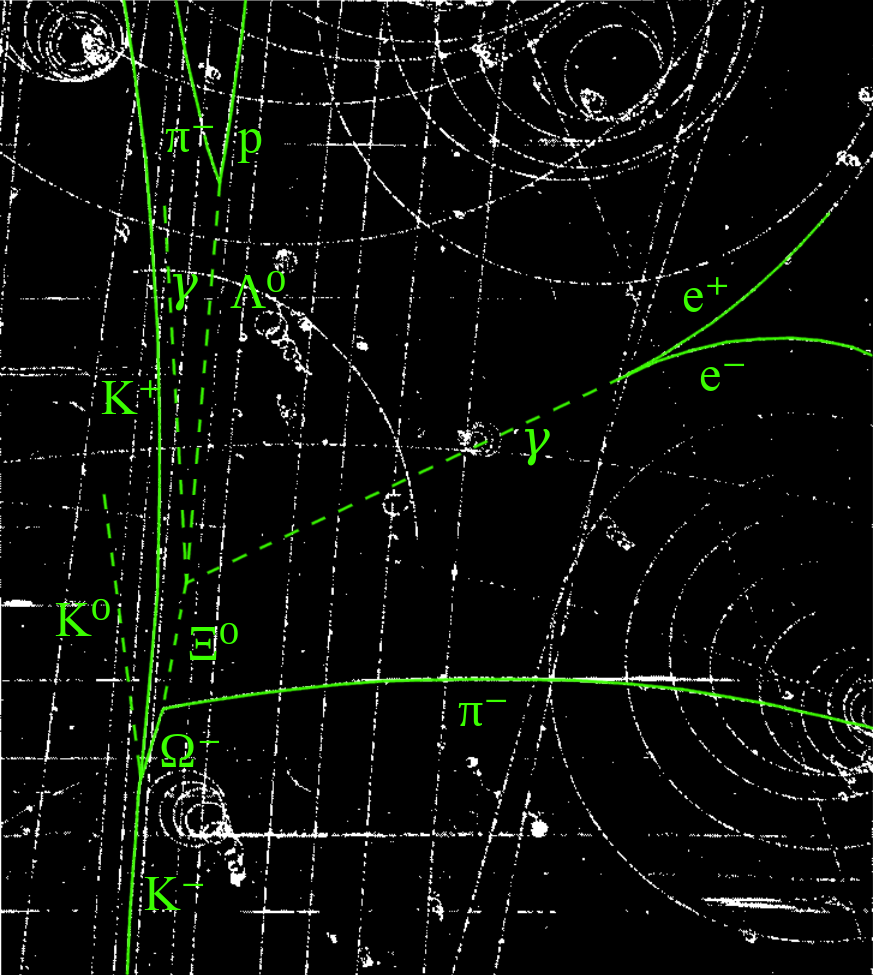
\includegraphics[width=\linewidth]{omega-minus-2.png}}
\column{0.52\linewidth}

\begin{center}
\begin{onlyenv}<1>
This is a famous photo: the 1964 discovery of the $\Omega$ baryon.

\vspace{1 cm}
Do you see it?

\vspace{1 cm}
\end{onlyenv}\begin{onlyenv}<2>
How about now?

\vspace{0.5 cm}
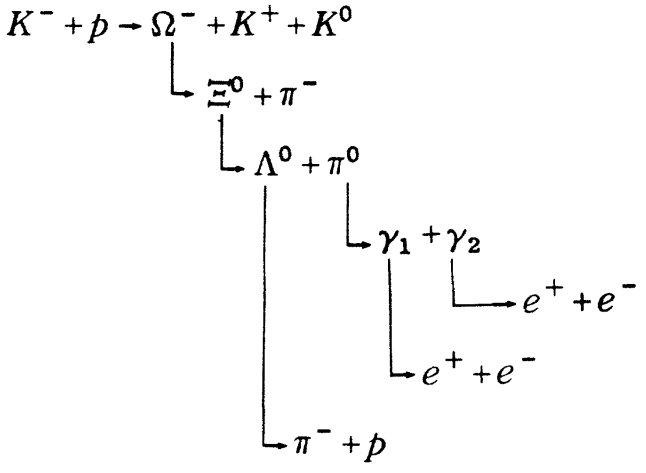
\includegraphics[width=\linewidth]{decay-chain.png}

\vspace{0.5 cm}
%% \begin{align*}
%% K^- + p & \to \Omega^- + K^+ + K^0 \\
%% \Omega^- & \to \Xi^0 + \pi^- \\
%% \Xi^0 & \to \Lambda^0 + \pi^0 \\
%% \Lambda^0 & \to p + \pi^- \\
%% \pi^0 & \to \gamma + \gamma
%% \end{align*}

\end{onlyenv}\begin{onlyenv}<3>
This is what particle physicists do: collide particles, produce new ones and take pictures of the decays.

\vspace{1 cm}
However, these pictures come to us unlabeled: lots of interactions overlap the ``interesting'' ones.

\vspace{1 cm}
\end{onlyenv}
\end{center}

\end{columns}
\end{frame}

\begin{frame}{}
\begin{columns}
\column{1.15\linewidth}
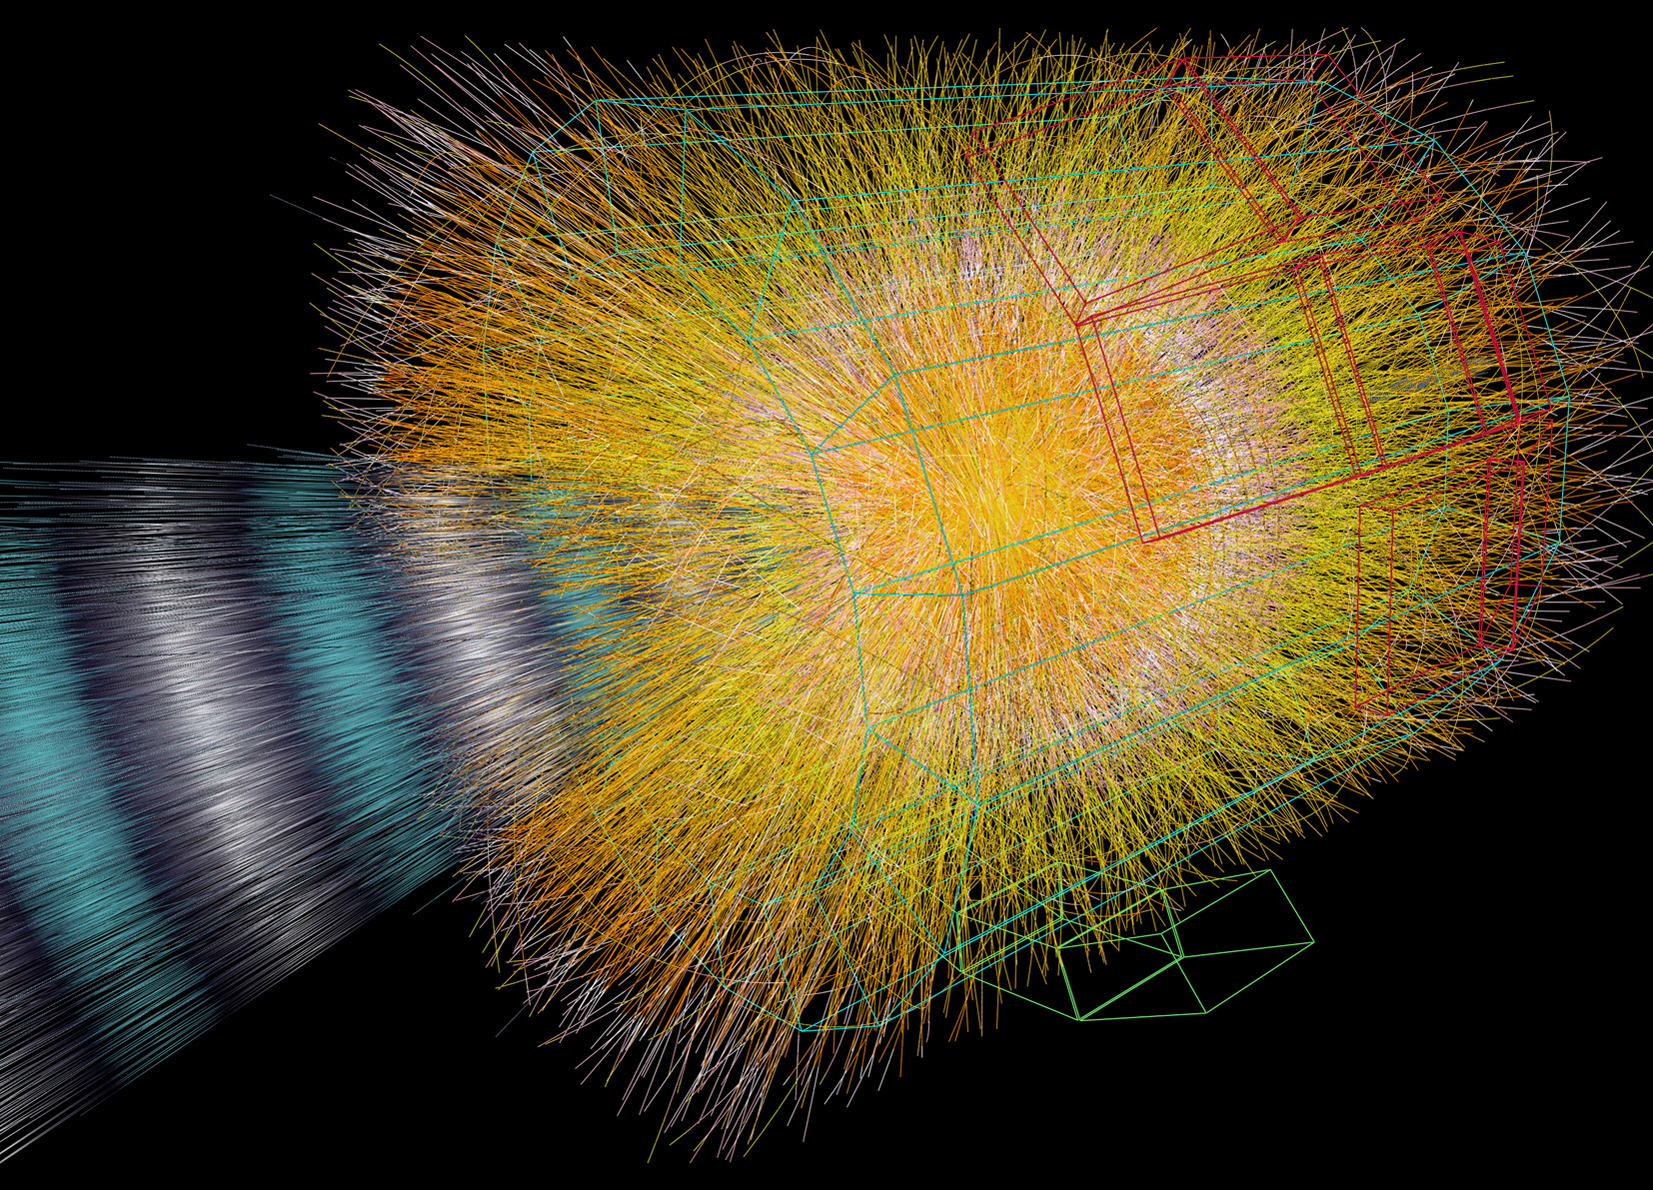
\includegraphics[width=\linewidth]{090324_ALICE-hirez.jpg}
\end{columns}
\end{frame}

\begin{frame}{Modern particle physics scales this up}
\vspace{0.15 cm}
\begin{columns}
\column{0.32\linewidth}
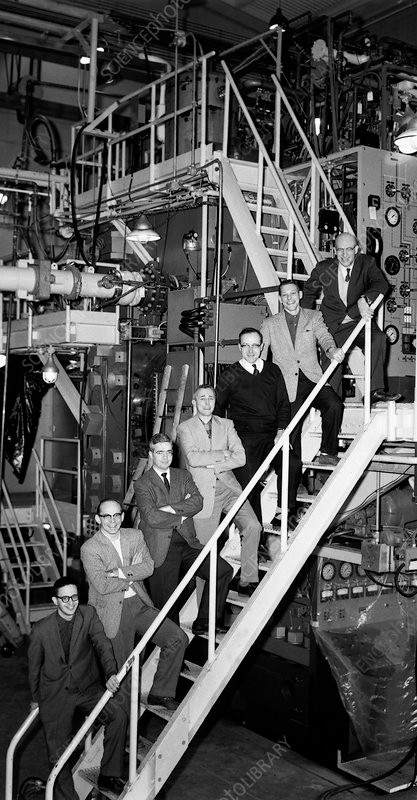
\includegraphics[width=\linewidth]{H4000010-Team_that_discovered_Omega_minus_particle.jpg}

\column{0.5\linewidth}
\begin{center}
\begin{columns}
\column{0.35\linewidth}
\centering
photographs

\vspace{0.5 cm}
100,000 events

\vspace{0.5 cm}
manual/semi-automated scans

\column{0.35\linewidth}
\centering
digitized signals \\

\vspace{0.5 cm}
$\sim$trillion events \\

\vspace{0.5 cm}
algorithmic searches and machine learning
\end{columns}
\end{center}

\column{0.32\linewidth}
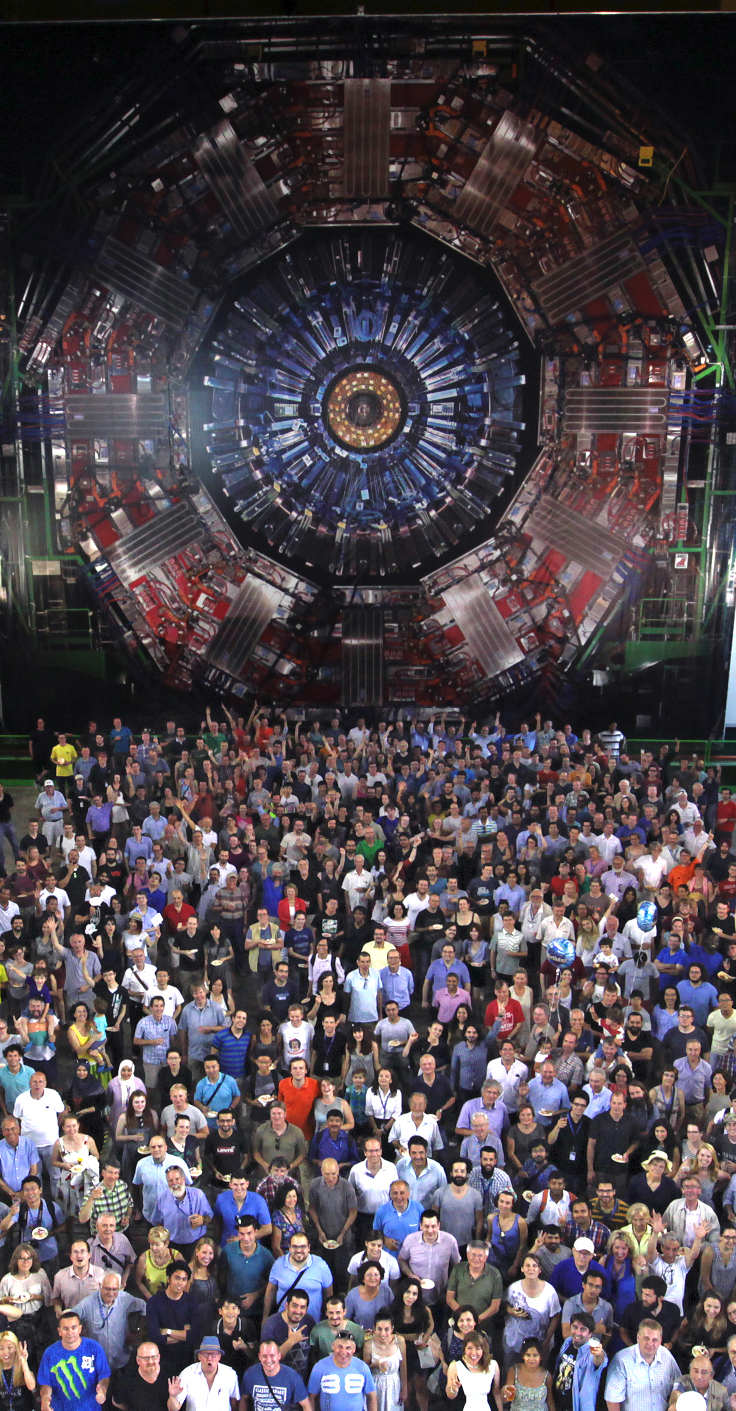
\includegraphics[width=\linewidth]{cms25_2.jpg}
\end{columns}
\end{frame}

\begin{frame}{Automatically identifying a particle decay}
\large
\vspace{0.5 cm}
\begin{enumerate}
\item Loop over all pairs of particle tracks, tentatively labeling them $\pi^+$ and $\pi^-$.
\item Calculate m = $\sqrt{(E_{\pi^+} + E_{\pi^-})^2 - \left|\vec{p}_{\pi^+} + \vec{p}_{\pi^-}\right|^2}$ for each pair.
\item The ones with $m \sim \mbox{mass}({K_s^0}) = 0.5\mbox{ GeV}/c^2$ are good candidates.
\end{enumerate}

\begin{center}
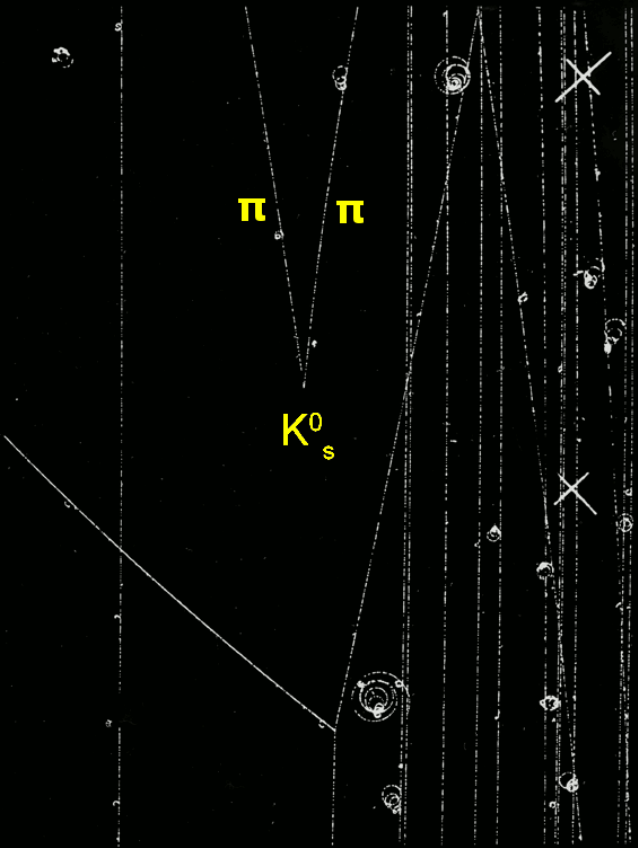
\includegraphics[height=4.2 cm]{kshort-1.png}\hspace{0.1 cm}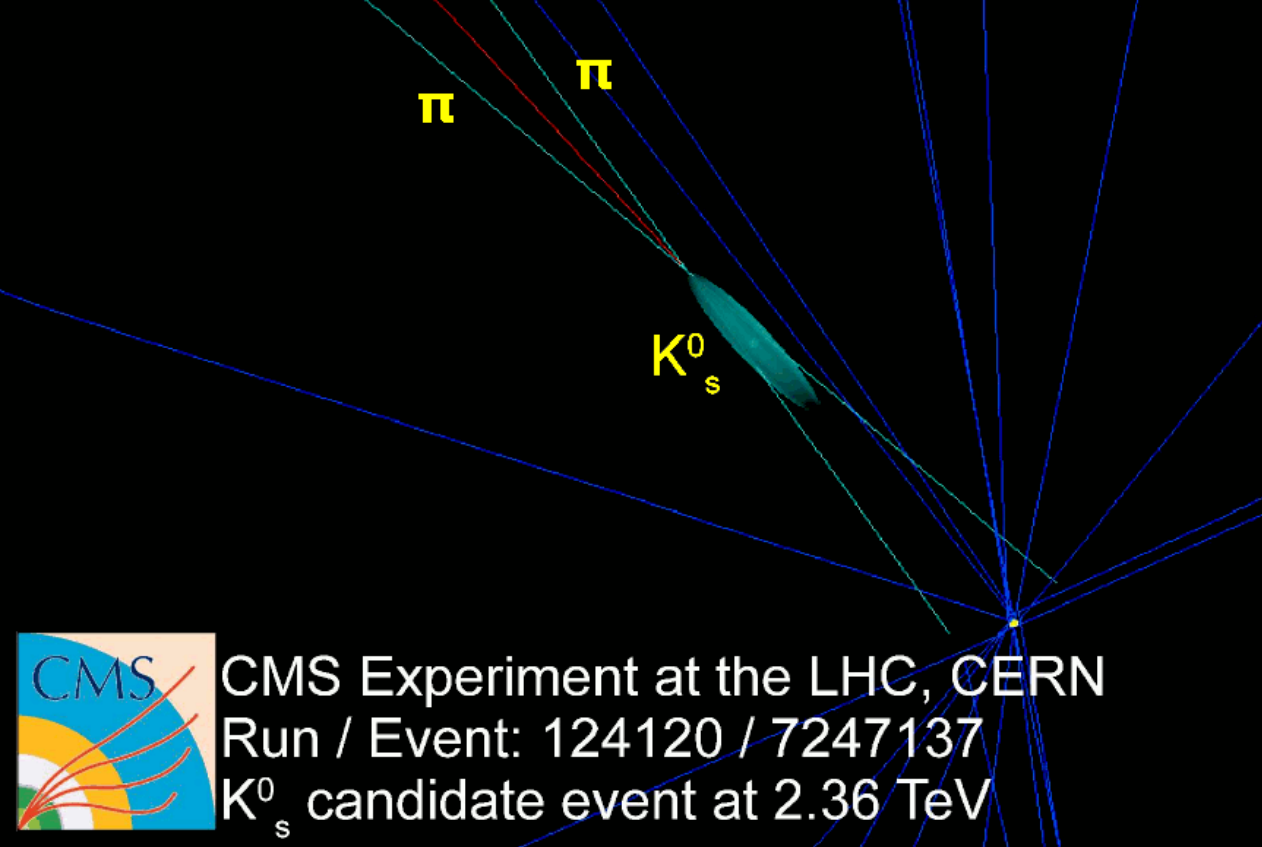
\includegraphics[height=4.2 cm]{kshort-2.png}\hspace{0.1 cm}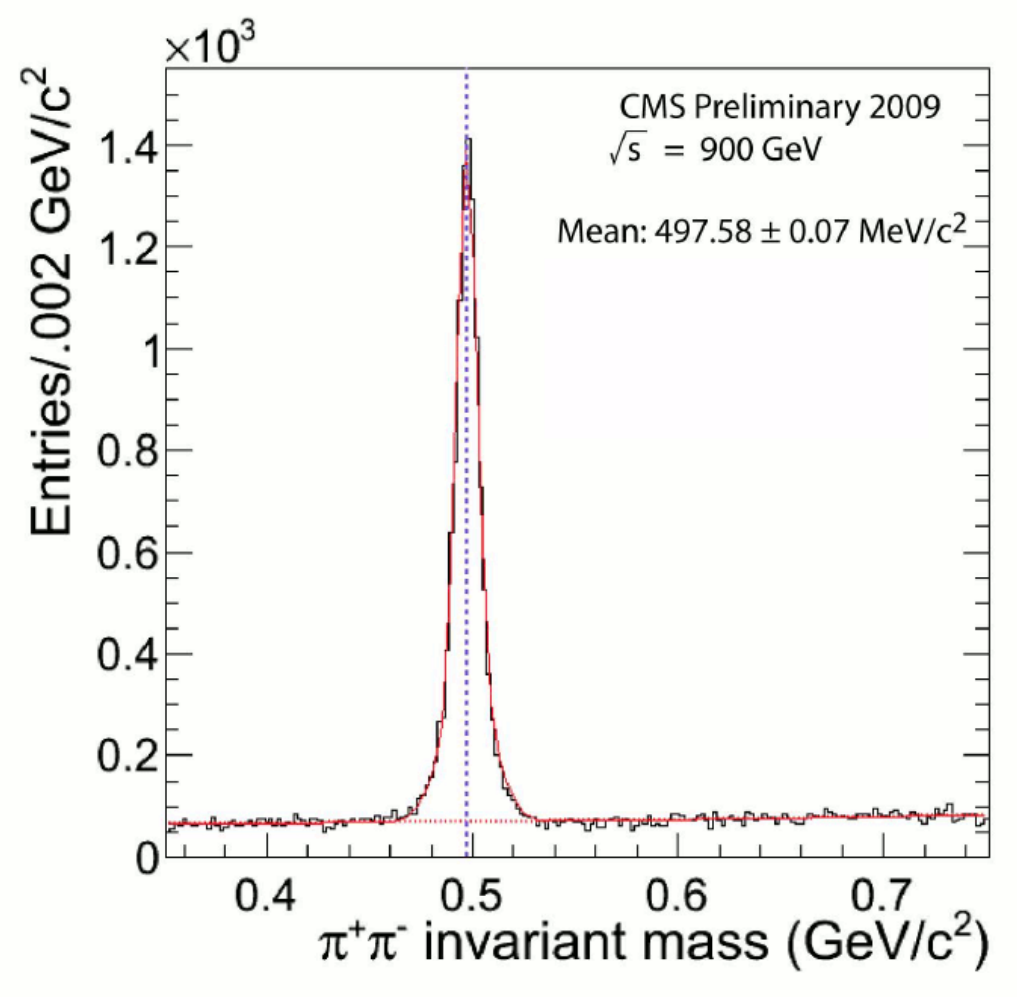
\includegraphics[height=4.2 cm]{kshort-3.png}
\end{center}
\end{frame}

\begin{frame}{Apply this technique successively down the decay chain}
\Large
\begin{center}
$H \to ZZ$\hspace{1 cm}$Z \to e^+e^-$\hspace{1 cm}$Z \to \mu^+\mu^-$
\end{center}

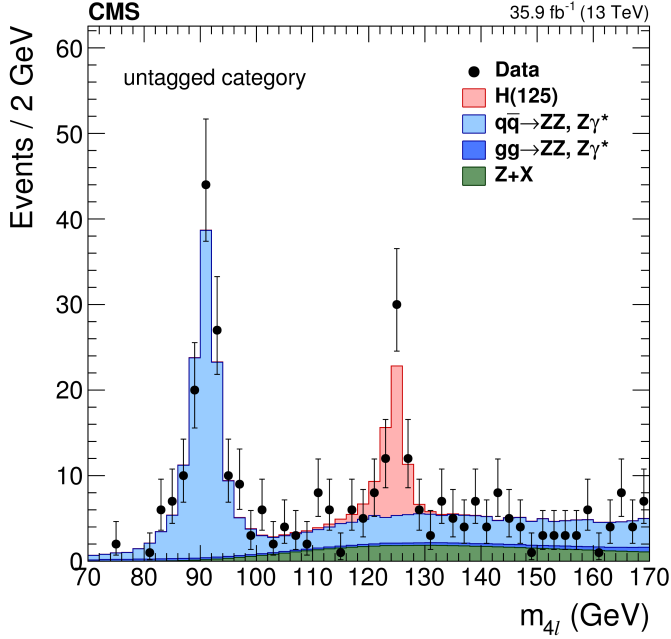
\includegraphics[height=6 cm]{higgs-to-four-leptons.png}\hfill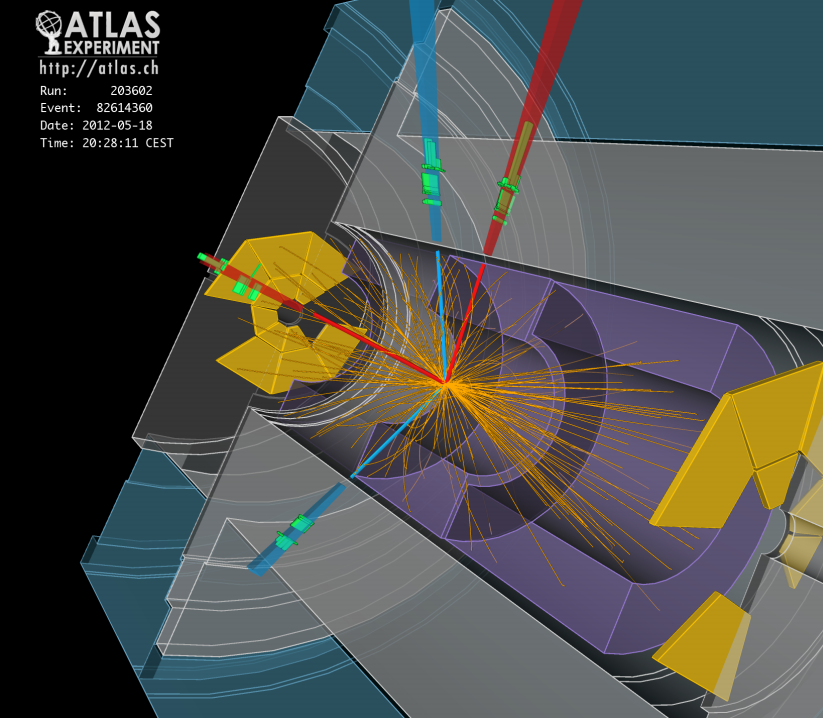
\includegraphics[height=6 cm]{higgs-to-four-leptons-2.png}
\end{frame}

\begin{frame}{From a computational point of view\ldots}
\Large
\vspace{0.25 cm}
\begin{itemize}\setlength{\itemsep}{0.25 cm}
\item All events are independent; no particles or decays cross from one event to the next \textcolor{gray}{(extremely few exceptions)}.
\item Detectors produce collections of different kinds of signals: tracks, energy deposition, timing, etc., each in its own variable-length collection.
\item Decay candidates may be thought of as a \mintinline{sql}{SELF JOIN}

(single collection) or a \mintinline{sql}{CROSS JOIN} (different collections) but always \mintinline{sql}{ON t1.eventId == t2.eventId}.
\item Good candidates are identified by {\it filtering} (throw away the bad) and/or {\it reduction} (pick the best of what remains.)
\end{itemize}
\end{frame}

\begin{frame}{From a computational point of view\ldots}
\Large
\vspace{0.5 cm}
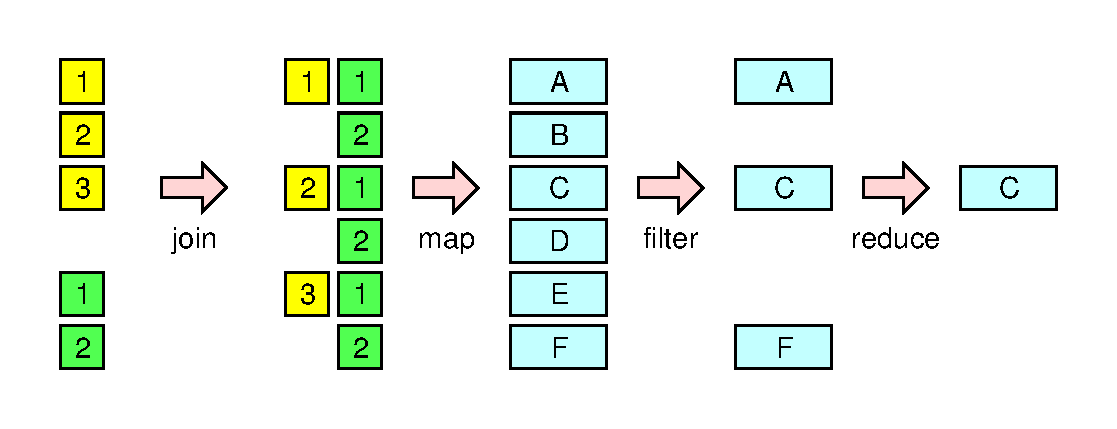
\includegraphics[width=\linewidth]{explode-flat-reduce.pdf}

\hfill \ldots independently for each event.
\end{frame}

\begin{frame}{From a computational point of view\ldots}
\Large
\vspace{0.25 cm}
\begin{itemize}
\item Large number of events, processed in parallel.
\item Each event has an {\it arbitrary number} of record structures.
\item Not reducible to a flat table without padding and/or loss.
\end{itemize}

\vspace{0.25 cm}
\begin{columns}
\column{0.5\linewidth}
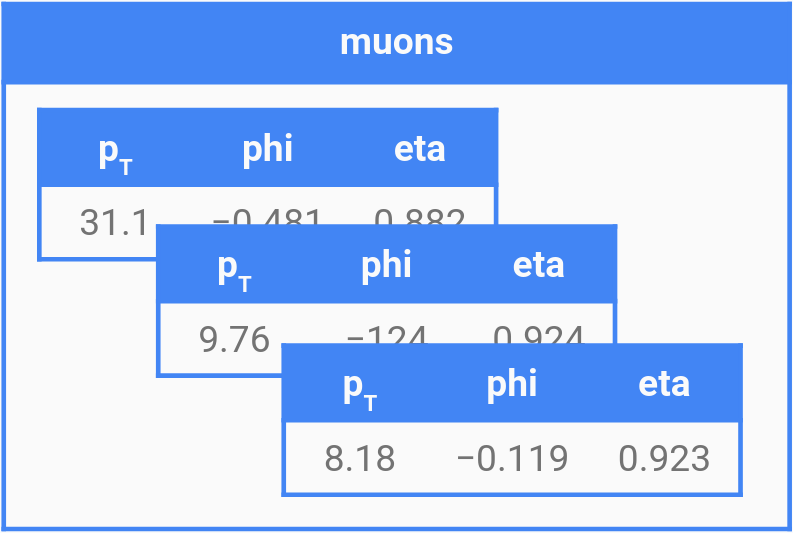
\includegraphics[width=\linewidth]{muons-as-objects.png}

\column{0.5\linewidth}
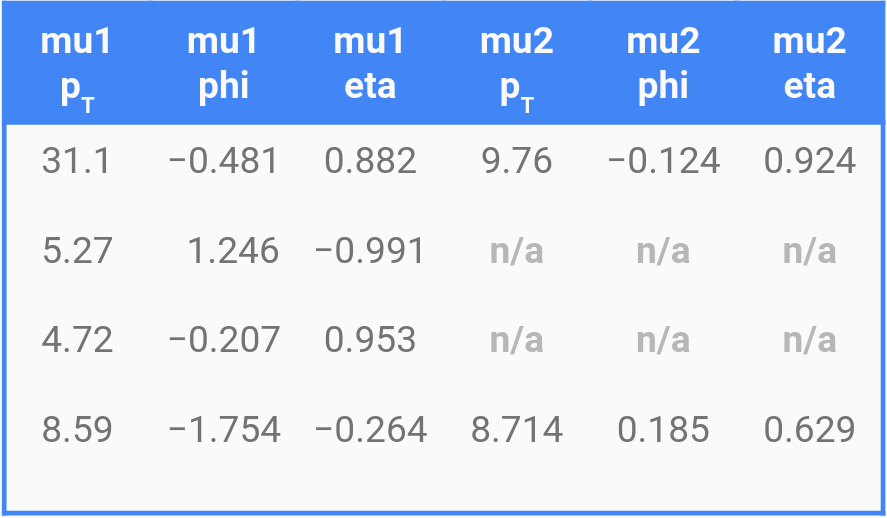
\includegraphics[width=\linewidth]{muons-as-a-table.png}
\end{columns}
\end{frame}

\begin{frame}{Programming languages used in particle physics}
\large
\vspace{0.5 cm}
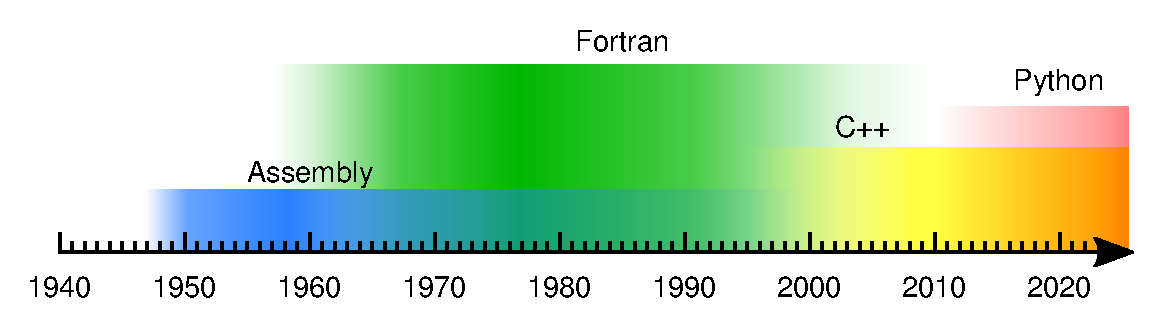
\includegraphics[width=\linewidth]{programming-languages.pdf}

\begin{itemize}\setlength{\itemsep}{0.2 cm}
\item First programmable computers were used for particle physics simulations.
\item Fortran was used to analyze events soon after the language was invented;

physicists wrote packages (BOS, HYDRA, ZBOOK) to add data structures.

\item Major transition from Fortran to C++ in the late 1990's/early 2000's.
\item Very recent adoption of Python (alongside C++).
\end{itemize}
\end{frame}

\begin{frame}{The Python transition is happening {\it right now}}
\vspace{0.2 cm}
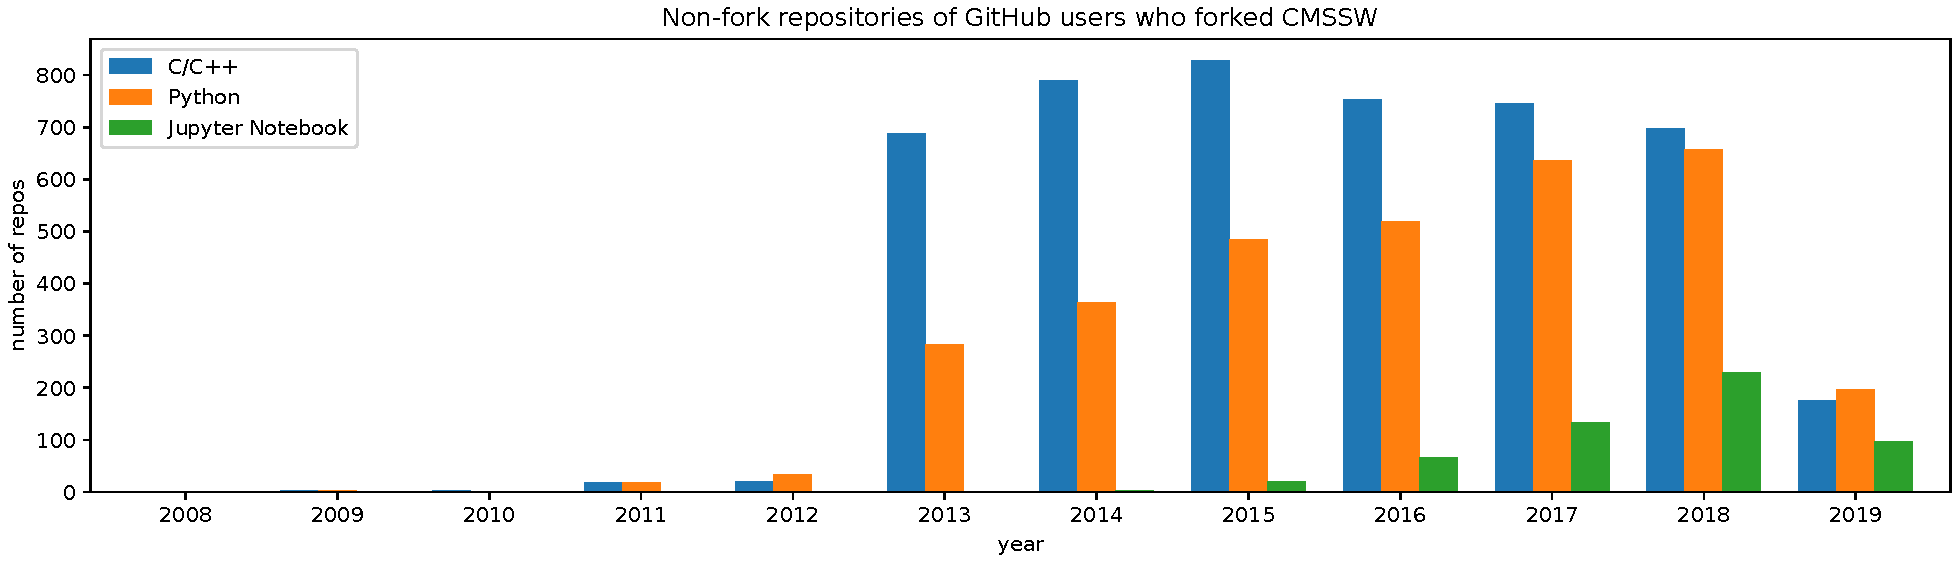
\includegraphics[width=\linewidth]{github-cmssw-lin.pdf}

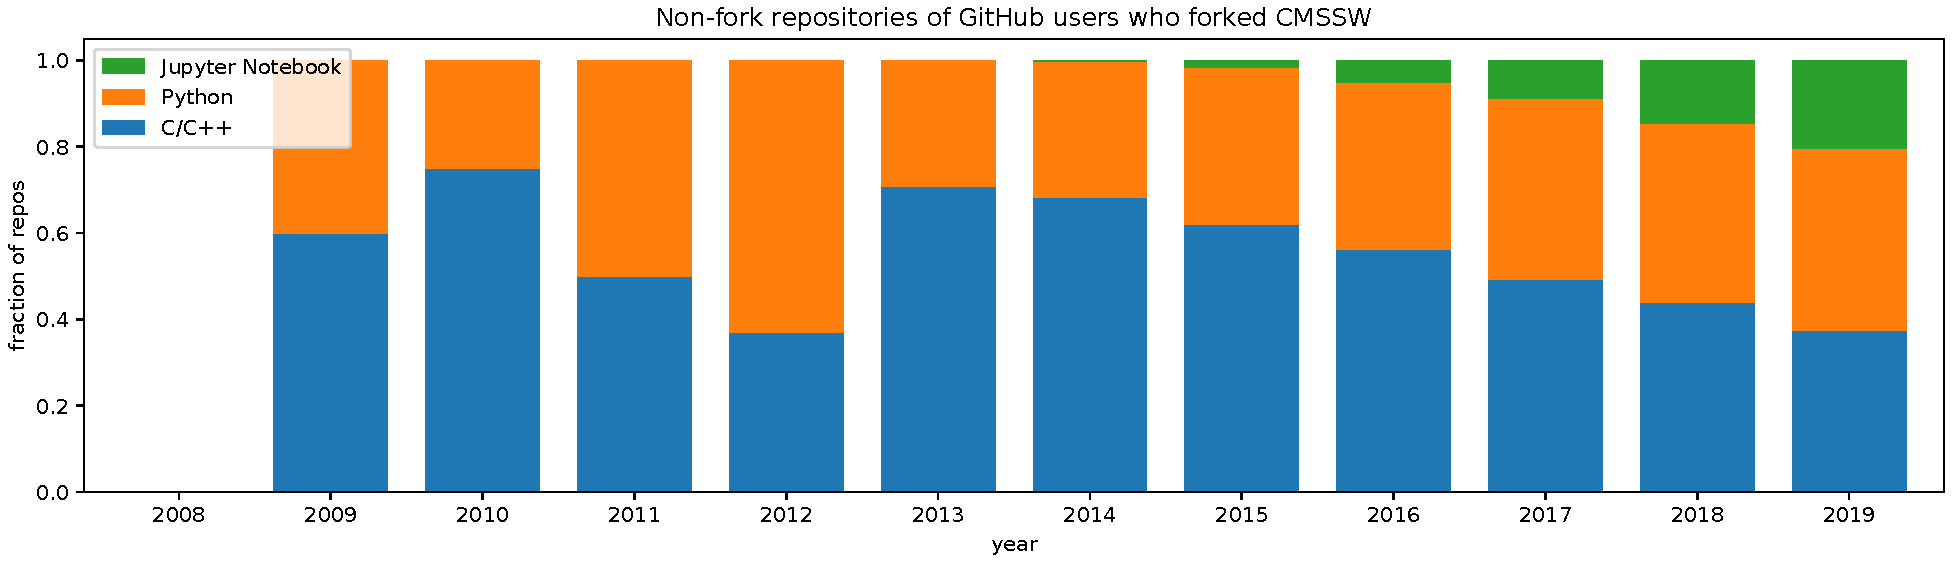
\includegraphics[width=\linewidth]{github-cmssw-frac.pdf}
\end{frame}

\begin{frame}[fragile]{In our field, ``conventional'' analysis means C++}
\vspace{0.25 cm}
\begin{columns}[b]
\column{0.7\linewidth}
\begin{minted}{c++}
std::vector<Kaon*> getKaons(Event event) {
  std::vector<Track*> tracks = event.getTracks();
  std::vector<Kaon*> kaons;
  for (auto t1 = tracks.begin(); t1 != tracks.end(); ++t1) {
    for (auto t2 = t1 + 1; t2 != tracks.end(); ++t2) {
      if (t1->charge != t2->charge) {
        double m = mass(t1, t2);
        if (fabs(m - 0.5) < 0.01) {
          kaons.push_back(new Kaon(t1, t2));
        }
      }
    }
  }
  return kaons;
}
\end{minted}

\vspace{0.1 cm}

\column{0.25\linewidth}
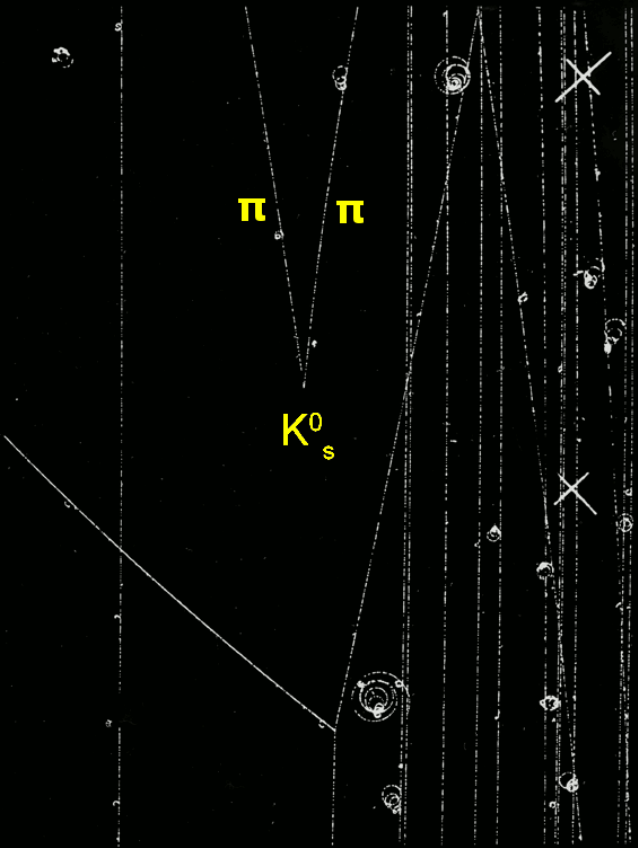
\includegraphics[width=\linewidth]{kshort-1.png}
\end{columns}
\end{frame}

\begin{frame}[fragile]{But direct translation to Python would be a performance disaster}
\vspace{0.25 cm}
\begin{columns}[b]
\column{0.7\linewidth}
\begin{minted}[stripnl=false]{python}
def getKaons(event):
  tracks = event.getTracks()
  kaons = []
  for i, t1 in enumerate(tracks):
    for t2 in tracks[i + 1:]:
      if t1.charge != t2.charge:
        m = mass(t1, t2)
        if abs(m - 0.5) < 0.01:
          kaons.append(Kaon(t1, t2))




  return kaons

\end{minted}

\vspace{0.1 cm}

\column{0.25\linewidth}
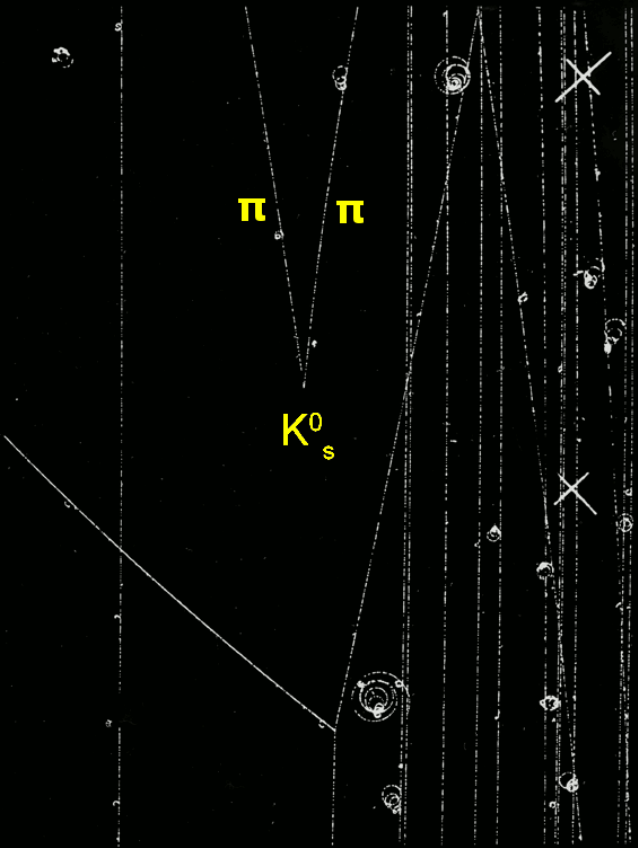
\includegraphics[width=\linewidth]{kshort-1.png}
\end{columns}
\end{frame}

\begin{frame}{High-performance processing in Python usually requires Numpy}
\vspace{0.5 cm}
\begin{center}

\includegraphics[width=0.35\linewidth]{numpy-logo.png}

\vspace{1 cm}
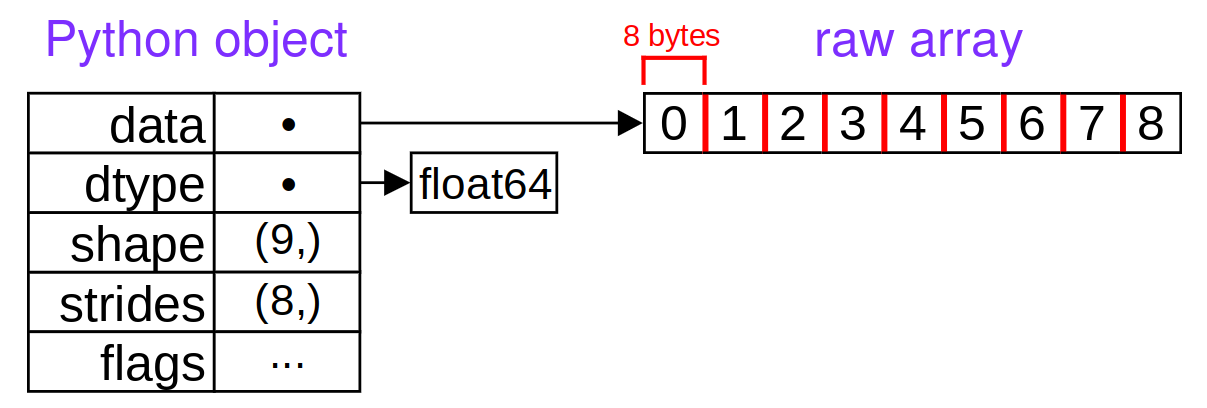
\includegraphics[width=0.75\linewidth]{numpy-memory-layout.png}
\end{center}
\end{frame}

\begin{frame}[fragile]{High-performance processing in Python usually requires Numpy}
\Large
\vspace{0.5 cm}
\begin{columns}
\column{0.52\linewidth}
Numpy has a suite of operations that each apply to whole arrays (compiled, maybe vectorized loop):

\small
\begin{minted}{python}
def calculate(pt, eta):
    pz = pt * numpy.sinh(eta)

calculate(pt_scalar, eta_scalar)
calculate(pt_array,  eta_array)
\end{minted}

\Large
\vspace{0.5 cm}

\uncover<2->{By manipulating the {\tt shape} and {\tt strides}, slices are $\mathcal{O}(1)$ and zero-copy.}

\column{0.4\linewidth}
\uncover<2->{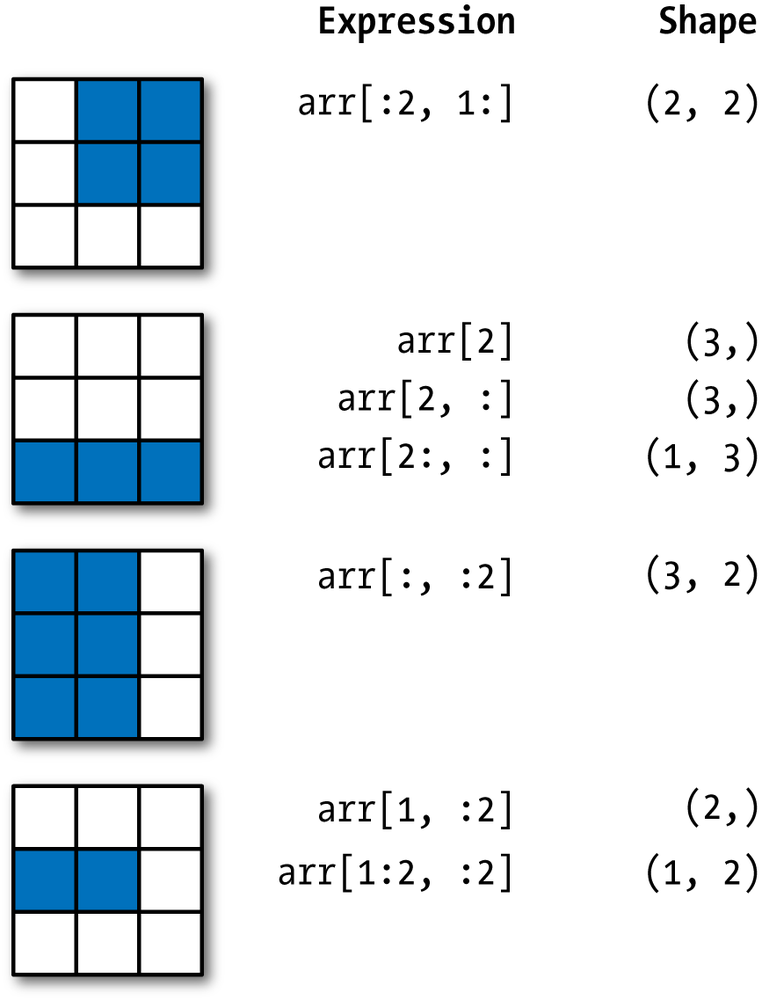
\includegraphics[width=\linewidth]{numpy-slicing.png}}
\end{columns}
\end{frame}

\begin{frame}{But Numpy doesn't have anything for unequal-length lists}
\Large
\vspace{0.05 cm}
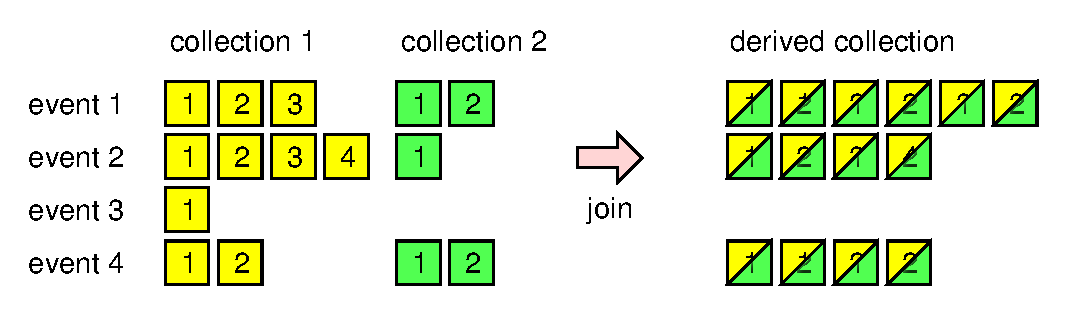
\includegraphics[width=\linewidth]{two-collections.pdf}

\vspace{-0.15 cm}
\uncover<2->{Some libraries* can represent arrays of unequal-length arrays, known as ``jagged'' or ``ragged'' arrays.}

\vspace{0.15 cm}
\large
\uncover<2->{\textcolor{gray}{*Apache Arrow, XND, Zarr, TensorFlow, and ROOT (particle physics)}}
\end{frame}

\begin{frame}[fragile]{Jagged/nested data can be contiguous by field (``columnar'')}
\vspace{0.5 cm}
\begin{columns}
\column{0.5\linewidth}
\small
\begin{Verbatim}[commandchars=\\\{\}]
[[Muon(\textcolor{darkgreen}{31.1}, \textcolor{darkorange}{-0.481}, \textcolor{blue}{0.882}),
      Muon(\textcolor{darkgreen}{9.76}, \textcolor{darkorange}{-0.124}, \textcolor{blue}{0.924}),
      Muon(\textcolor{darkgreen}{8.18}, \textcolor{darkorange}{-0.119}, \textcolor{blue}{0.923})],
 [Muon(\textcolor{darkgreen}{5.27}, \textcolor{darkorange}{1.246}, \textcolor{blue}{-0.991})],
 [Muon(\textcolor{darkgreen}{4.72}, \textcolor{darkorange}{-0.207}, \textcolor{blue}{0.953})],
 [Muon(\textcolor{darkgreen}{8.59}, \textcolor{darkorange}{-1.754}, \textcolor{blue}{-0.264}),
      Muon(\textcolor{darkgreen}{8.714}, \textcolor{darkorange}{0.185}, \textcolor{blue}{0.629})]
]
\end{Verbatim}
\column{0.35\linewidth}
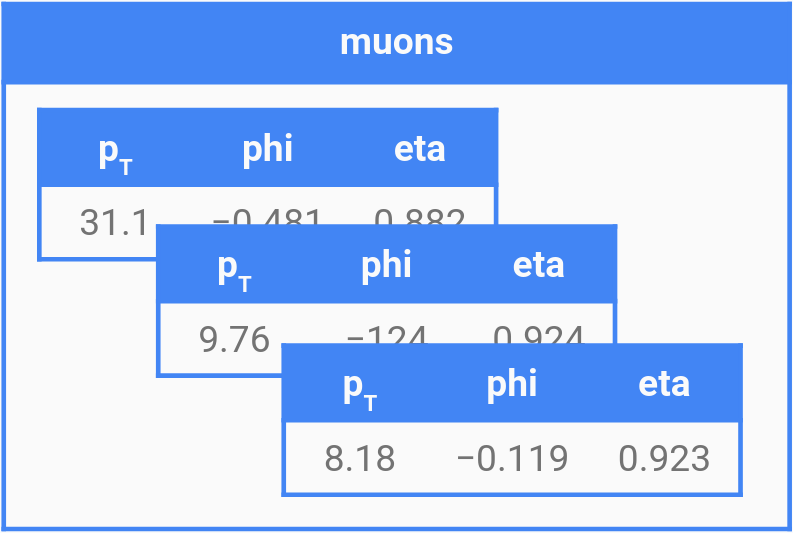
\includegraphics[width=\linewidth]{muons-as-objects.png}
\end{columns}
\vspace{0.5 cm}
\large The trick: represent structure with \only<1>{\textcolor{red}{counts}}\only<2,3,4>{counts} or \only<2>{\textcolor{red}{offsets}}\only<1,3,4>{offsets} or \only<3>{\textcolor{red}{starts/stops}}\only<1,2,4>{starts/stops} or \only<4>{\textcolor{red}{parents}}\only<1,2,3>{parents}.
\vspace{0.25 cm}
\begin{tabular}{r l}
\only<1>{\small \textcolor{red}{counts}  & \textcolor{red}{\tt\scriptsize \ \ \ \ \ 3,\ \ \ \ \ \ \ \ \ \ \ \ \ \ \ \ \ \ \ \ \ \ 1,\ \ \ \ \ \ 1,\ \ \ \ \ \ 2\ \ \ \ \ \ \ \ \ } \\}
\only<2>{\small \textcolor{red}{offsets} & \textcolor{red}{\tt\scriptsize \ \ \ \ \ 0,\ \ \ \ \ \ \ \ \ \ \ \ \ \ \ \ \ \ \ \ \ \ 3,\ \ \ \ \ \ 4,\ \ \ \ \ \ 5,\ \ \ \ \ \ \ 7} \\}
\only<4>{\small \textcolor{red}{parents} & \textcolor{red}{\tt\scriptsize \ \ \ \ \ 0,\ \ \ \ \ \ 0,\ \ \ \ \ \ 0,\ \ \ \ \ \ 1,\ \ \ \ \ \ 2,\ \ \ \ \ \ 3,\ \ \ \ \ 3} \\}
\only<3>{\small \textcolor{red}{starts}  & \textcolor{red}{\tt\scriptsize \ \ \ \ \ 0,\ \ \ \ \ \ \ \ \ \ \ \ \ \ \ \ \ \ \ \ \ \ 3,\ \ \ \ \ \ 4,\ \ \ \ \ \ 5\ \ \ \ \ \ \ \ \ } \\}
\uncover<3>{\small \textcolor{red}{stops}   & \textcolor{red}{\tt\scriptsize \ \ \ \ \ 3,\ \ \ \ \ \ \ \ \ \ \ \ \ \ \ \ \ \ \ \ \ \ 4,\ \ \ \ \ \ 5,\ \ \ \ \ \ 7\ \ \ \ \ \ \ \ \ } \\}
\small \mbox{\hspace{1 cm}$p_T$} & \textcolor{darkgreen}{\tt\scriptsize \ \ 31.1,\ \ \ 9.76,\ \ \ 8.18,\ \ \ 5.27,\ \ \ 4.72,\ \ \ 8.59, 8.714} \\
\small phi &  \textcolor{darkorange}{\tt\scriptsize -0.481,\ -0.123,\ -0.119,\ \ 1.246,\ -0.207,\ -1.754,\ 0.185} \\
\small eta &        \textcolor{blue}{\tt\scriptsize \ 0.882,\ \ 0.924,\ \ 0.923,\ -0.991,\ \ 0.953,\ -0.264,\ 0.629} \\
\end{tabular}
\end{frame}

\begin{frame}{}
\LARGE
\vspace{1 cm}
\begin{center}
But we can go beyond {\it representing} columnar jagged arrays and {\it manipulate} them in this form
\end{center}
\end{frame}

\begin{frame}[fragile]{Example of a jagged operation: manipulating jagged arrays}
\vspace{0.5 cm}
\textcolor{red}{``Remove the first muon from each event.''} \uncover<2->{\textcolor{red}{\bf$\longrightarrow$ rewrite all inner lists.}}
\scriptsize
\begin{onlyenv}<1>
\begin{Verbatim}[commandchars=\\\{\}]
[[Muon(\textcolor{darkgreen}{31.1}, \textcolor{darkorange}{-0.481}, \textcolor{blue}{0.882}), Muon(\textcolor{darkgreen}{9.76}, \textcolor{darkorange}{-0.124}, \textcolor{blue}{0.924}), Muon(\textcolor{darkgreen}{8.18}, \textcolor{darkorange}{-0.119}, \textcolor{blue}{0.923})],
 [Muon(\textcolor{darkgreen}{5.27}, \textcolor{darkorange}{1.246}, \textcolor{blue}{-0.991})],
 [Muon(\textcolor{darkgreen}{4.72}, \textcolor{darkorange}{-0.207}, \textcolor{blue}{0.953})],
 [Muon(\textcolor{darkgreen}{8.59}, \textcolor{darkorange}{-1.754}, \textcolor{blue}{-0.264}), Muon(\textcolor{darkgreen}{8.714}, \textcolor{darkorange}{0.185}, \textcolor{blue}{0.629})],
 ...
\end{Verbatim}
\end{onlyenv}\begin{onlyenv}<2->
\begin{Verbatim}[commandchars=\\\{\}]
[[     \textcolor{darkgreen}{    }  \textcolor{darkorange}{      }  \textcolor{blue}{     }   Muon(\textcolor{darkgreen}{9.76}, \textcolor{darkorange}{-0.124}, \textcolor{blue}{0.924}), Muon(\textcolor{darkgreen}{8.18}, \textcolor{darkorange}{-0.119}, \textcolor{blue}{0.923})],
 [     \textcolor{darkgreen}{    }  \textcolor{darkorange}{     }  \textcolor{blue}{      } ],
 [     \textcolor{darkgreen}{    }  \textcolor{darkorange}{      }  \textcolor{blue}{     } ],
 [     \textcolor{darkgreen}{    }  \textcolor{darkorange}{      }  \textcolor{blue}{      }   Muon(\textcolor{darkgreen}{8.714}, \textcolor{darkorange}{0.185}, \textcolor{blue}{0.629})],
 ...
\end{Verbatim}
\end{onlyenv}
\normalsize
\vspace{0.5 cm}
\textcolor{red}{``Remove the first muon from each event.''} \uncover<2->{\textcolor{red}{\bf$\longrightarrow$ increase all starts by 1.}}
\vspace{0.25 cm}
\begin{onlyenv}<1>
\begin{tabular}{r l}
\small starts  &                    {\tt\scriptsize \ \ \ \ \ 0,\ \ \ \ \ \ \ \ \ \ \ \ \ \ \ \ \ \ \ \ \ \ 3,\ \ \ \ \ \ 4,\ \ \ \ \ \ 5\ \ \ \ \ \ \ \ \ } \\
\small stops   &                    {\tt\scriptsize \ \ \ \ \ 3,\ \ \ \ \ \ \ \ \ \ \ \ \ \ \ \ \ \ \ \ \ \ 4,\ \ \ \ \ \ 5,\ \ \ \ \ \ 7\ \ \ \ \ \ \ \ \ } \\
\small $p_T$ & \textcolor{darkgreen}{\tt\scriptsize \ \ 31.1,\ \ \ 9.76,\ \ \ 8.18,\ \ \ 5.27,\ \ \ 4.72,\ \ \ 8.59, 8.714} \\
\small phi &  \textcolor{darkorange}{\tt\scriptsize -0.481,\ -0.123,\ -0.119,\ \ 1.246,\ -0.207,\ -1.754,\ 0.185} \\
\small eta &        \textcolor{blue}{\tt\scriptsize \ 0.882,\ \ 0.924,\ \ 0.923,\ -0.991,\ \ 0.953,\ -0.264,\ 0.629} \\
\end{tabular}
\end{onlyenv}\begin{onlyenv}<2->
\begin{tabular}{r l}
\small starts  &     \textcolor{red}{\tt\scriptsize \ \ \ \ \ 1,\ \ \ \ \ \ \ \ \ \ \ \ \ \ \ \ \ \ \ \ \ \ 4,\ \ \ \ \ \ 5,\ \ \ \ \ \ 6\ \ \ \ \ \ \ \ \ } \\
\small stops   &                    {\tt\scriptsize \ \ \ \ \ 3,\ \ \ \ \ \ \ \ \ \ \ \ \ \ \ \ \ \ \ \ \ \ 4,\ \ \ \ \ \ 5,\ \ \ \ \ \ 7\ \ \ \ \ \ \ \ \ } \\
\small $p_T$ & \textcolor{darkgreen}{\tt\scriptsize \ \ 31.1,\ \ \ 9.76,\ \ \ 8.18,\ \ \ 5.27,\ \ \ 4.72,\ \ \ 8.59, 8.714} \\
\small phi &  \textcolor{darkorange}{\tt\scriptsize -0.481,\ -0.123,\ -0.119,\ \ 1.246,\ -0.207,\ -1.754,\ 0.185} \\
\small eta &        \textcolor{blue}{\tt\scriptsize \ 0.882,\ \ 0.924,\ \ 0.923,\ -0.991,\ \ 0.953,\ -0.264,\ 0.629} \\
\end{tabular}\end{onlyenv}
\vspace{0.25 cm}

\large
\uncover<3>{We didn't need to touch any contents (i.e.\ read from disk/decompress them).}

\vspace{0.25 cm}
\uncover<3>{Can be very useful if only $\sim$10\% of the fields are of interest!}
\end{frame}

\begin{frame}{}
\Large
\vspace{1 cm}
\begin{itemize}\setlength{\itemsep}{0.5 cm}
\item<1-> Columnar data structures are {\it fully composable:} a jagged array's content can be another jagged array, some fields of a record structure can be jagged, others not.
\item<2-> Most operations (such as slicing) can modify the structure ({\tt counts}/{\tt offsets}/{\tt starts,stops}/{\tt parents}) without touching the nested content.
\end{itemize}
\end{frame}

%% \begin{frame}{Example: generate distinct muon pairs}
%% \vspace{0.2 cm}

%% \begin{columns}
%% \column{1.1\linewidth}

%% {\large\bf muons:}

%% \vspace{0.2 cm}
%% \begin{tabular}{r l}
%% \textcolor{red}{counts}  & \textcolor{red}{\tt \ \ \ \ \ 3,\ \ \ \ \ \ \ \ \ \ \ \ \ \ \ \ \ \ \ \ \ \ 1,\ \ \ \ \ \ 1,\ \ \ \ \ \ 2\ \ \ \ \ \ \ \ \ } \\
%% \textcolor{red}{offsets} & \textcolor{red}{\tt \ \ \ \ \ 0,\ \ \ \ \ \ \ \ \ \ \ \ \ \ \ \ \ \ \ \ \ \ 3,\ \ \ \ \ \ 4,\ \ \ \ \ \ 5,\ \ \ \ \ \ \ 7} \\
%% \textcolor{red}{starts}  & \textcolor{red}{\tt \ \ \ \ \ 0,\ \ \ \ \ \ \ \ \ \ \ \ \ \ \ \ \ \ \ \ \ \ 3,\ \ \ \ \ \ 4,\ \ \ \ \ \ 5\ \ \ \ \ \ \ \ \ } \\
%% \textcolor{red}{stops}   & \textcolor{red}{\tt \ \ \ \ \ 3,\ \ \ \ \ \ \ \ \ \ \ \ \ \ \ \ \ \ \ \ \ \ 4,\ \ \ \ \ \ 5,\ \ \ \ \ \ 7\ \ \ \ \ \ \ \ \ } \\
%% \mbox{\hspace{1 cm}$p_T$} & \textcolor{darkgreen}{\tt \ \ 31.1,\ \ \ 9.76,\ \ \ 8.18,\ \ \ 5.27,\ \ \ 4.72,\ \ \ 8.59, 8.714} \\
%% phi &  \textcolor{darkorange}{\tt -0.481,\ -0.123,\ -0.119,\ \ 1.246,\ -0.207,\ -1.754,\ 0.185} \\
%% eta &        \textcolor{blue}{\tt \ 0.882,\ \ 0.924,\ \ 0.923,\ -0.991,\ \ 0.953,\ -0.264,\ 0.629} \\
%% \end{tabular}

%% \vspace{0.6 cm}
%% {\large\bf muons.choose(2):}

%% \vspace{0.2 cm}
%% \begin{tabular}{r l}
%% \textcolor{red}{counts}  &   \textcolor{red}{\tt 3,\ \ \ \ \ \ \ 0,\ 0,\ 1} \\
%% \textcolor{red}{offsets} &   \textcolor{red}{\tt 0,\ \ \ \ \ \ \ 2,\ 2,\ 2,\ 3} \\
%% \textcolor{black}{left}  & \textcolor{black}{\tt 0,\ 0,\ 1,\ \ \ \ \ \ \ 5} \\
%% \textcolor{black}{right} & \textcolor{black}{\tt 1,\ 2,\ 2,\ \ \ \ \ \ \ 6} \\
%% \textcolor{black}{left.content}  & \textcolor{black}{muons} \\
%% \textcolor{black}{right.content} & \textcolor{black}{muons} \\
%% \end{tabular}

%% \vspace{-3.2 cm}
%% \uncover<2->{\hfill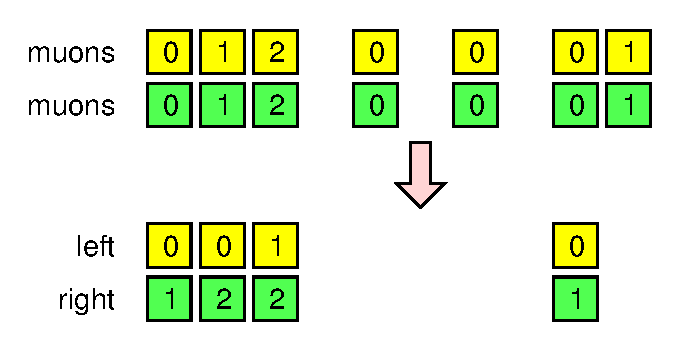
\includegraphics[height=3.5 cm]{muons-choose-2.pdf}}

%% \vspace{0.2 cm}
%% \uncover<3->{\textcolor{gray}{(The ``left'' and ``right'' of each pair is a link to the original muons.)}}
%% \end{columns}
%% \end{frame}

%% \begin{frame}[fragile]{As a data structure}
%% \vspace{0.25 cm}
%% \begin{columns}
%% \column{1.08\linewidth}
%% \scriptsize
%% \begin{verbatim}
%% muons =
%%     ListArray(
%%         offsets = [0, 3, 4, 5, 7],
%%         content =
%%             RecordArray(
%%                  pT = numpy.array([  31.1,   9.76,   8.18,   5.27,   4.72,   8.59, 8.714]),
%%                 eta = numpy.array([-0.481, -0.123, -0.119,  1.246, -0.207, -1.754, 0.185]),
%%                 phi = numpy.array([ 0.882,  0.924,  0.923, -0.991,  0.953, -0.264, 0.629])))



%% muons.choose(2) =
%%     ListArray(
%%         offsets = [0, 2, 2, 2, 3],
%%         content =
%%             RecordArray(
%%                  left = IndirectArray(index = [0, 0, 1, 5], content = muons)
%%                 right = IndirectArray(index = [1, 2, 2, 6], content = muons)))
%% \end{verbatim}
%% \end{columns}
%% \end{frame}

\begin{frame}[fragile]{Awkward Array: jagged/nested data with a Numpy-like interface}
\vspace{0.35 cm}
\small
\hfill
\includegraphics[height=2 cm]{awkward-logo.pdf}

\vspace{-2 cm}
\begin{minted}{python}
>>> import awkward
>>> array = awkward.fromiter(
...     [[1.1, 2.2, None, 3.3, None],
...      [4.4, [5.5]],
...      [{"x": 6, "y": {"z": 7}}, None, {"x": 8, "y": {"z": 9}}]])
\end{minted}

\begin{uncoverenv}<2->
\begin{minted}{python}
>>> print(array)            # an array of typed data structures
[[1.1 2.2 None 3.3 None] [4.4 [5.5]] [<Row 0> None <Row 1>]]
\end{minted}
\end{uncoverenv}

\begin{uncoverenv}<3->
\begin{minted}{python}
>>> print(array[:, -2:])    # get whole outer list, last two of inner
[[3.3 None] [4.4 [5.5]] [None <Row 1>]]
\end{minted}
\end{uncoverenv}

\begin{uncoverenv}<4->
\begin{minted}{python}
>>> (array + 100).tolist()  # element-wise function applied to arrays
                            # i.e. a Numpy ufunc (all ufuncs work)
[[101.1, 102.2, None, 103.3, None],
 [104.4, [105.5]],
 [{'x': 106, 'y': {'z': 107}}, None, {'x': 108, 'y': {'z': 109}}]]
\end{minted}
\end{uncoverenv}
\end{frame}

\begin{frame}[fragile]{Internally, it's a bunch or Numpy arrays {\it interpreted} as nested data}
\begin{columns}
\column{1.1\linewidth}
\scriptsize
\begin{minted}{python}
>>> array.layout
 layout
[           ()] JaggedArray(starts=layout[0], stops=layout[1], content=layout[2])
[            0]   ndarray(shape=3, dtype=dtype('int64'))
[            1]   ndarray(shape=3, dtype=dtype('int64'))
[            2]   IndexedMaskedArray(mask=layout[2, 0], content=layout[2, 1], maskedwhen=-1)
[         2, 0]     ndarray(shape=10, dtype=dtype('int64'))
[         2, 1]     UnionArray(tags=layout[2, 1, 0], index=layout[2, 1, 1],
                               contents=[layout[2, 1, 2], layout[2, 1, 3], layout[2, 1, 4]])
[      2, 1, 0]       ndarray(shape=7, dtype=dtype('uint8'))
[      2, 1, 1]       ndarray(shape=7, dtype=dtype('int64'))
[      2, 1, 2]       ndarray(shape=4, dtype=dtype('float64'))
[      2, 1, 3]       JaggedArray(starts=layout[2, 1, 3, 0], stops=layout[2, 1, 3, 1],
                                  content=layout[2, 1, 3, 2])
[   2, 1, 3, 0]         ndarray(shape=1, dtype=dtype('int64'))
[   2, 1, 3, 1]         ndarray(shape=1, dtype=dtype('int64'))
[   2, 1, 3, 2]         ndarray(shape=1, dtype=dtype('float64'))
[      2, 1, 4]       Table(x=layout[2, 1, 4, 0], y=layout[2, 1, 4, 1])
[   2, 1, 4, 0]         ndarray(shape=2, dtype=dtype('int64'))
[   2, 1, 4, 1]         Table(z=layout[2, 1, 4, 1, 0])
[2, 1, 4, 1, 0]           ndarray(shape=2, dtype=dtype('int64'))
\end{minted}
\end{columns}
\end{frame}

\begin{frame}[fragile]{Array indexing is a function; arrays have functional type}
\small
\begin{minted}{python}
>>> # array type formatted to look like a curried function's type
>>> print(array.type)
[0, 3) -> [0, inf) -> ?((float64             |
                         [0, inf) -> float64 |
                         'x' -> int64
                         'y' -> 'z' -> int64 ))
\end{minted}

\normalsize
\vspace{0.5 cm}
{\bf How to read the above:}
\begin{itemize}
\item First square bracket in \mintinline{python}{array[x]} takes a non-negative integer less than 3.
\item Second takes a non-negative integer (unknown upper limit because it's jagged).
\item What that returns is nullable (might be \mintinline{python}{None}).
\item And it could be a \mintinline{python}{float}, a jagged array of floats, or a record taking \mintinline{python}{'x'} or \mintinline{python}{'y'}.
\item \mintinline{python}{'x'} returns an integer; \mintinline{python}{'y'} returns another record taking \mintinline{python}{'z'} to integers.
\end{itemize}
\end{frame}

\begin{frame}{}
\LARGE
\vspace{1 cm}
\begin{center}
Let's look at a real dataset in detail
\end{center}
\end{frame}

\begin{frame}[fragile]{NASA exoplanets dataset: stars may have more than one planet}
\begin{columns}
\column{1.09\linewidth}
\small
\begin{minted}{python}
>>> import urllib.request
>>> stars = awkward.fromiter(
...     json.load(
...         urllib.request.urlopen(
...            "http://scikit-hep.org/uproot/examples/exoplanets.json")))
\end{minted}

\begin{onlyenv}<1>
\begin{minted}{python}
>>> stars
<Table [<Row 0> <Row 1> <Row 2> ... <Row 2933> <Row 2934>]>
\end{minted}

\vspace{10 cm}
\end{onlyenv}
\begin{onlyenv}<2>
\begin{minted}{python}
>>> stars[8:10].tolist()
[{'name': '24 Sex', 'ra': 155.86821, 'dec': -0.902244, 'dist': 72.21,
  'mass': 1.54, 'radius': 4.9, 'planets': [
      {'name': 'b', 'orbit': 1.333, 'eccen': 0.09, 'period': 452.8,
       'mass': 1.99, 'radius': None},
      {'name': 'c', 'orbit': 2.08, 'eccen': 0.29, 'period': 883.0,
       'mass': 0.86, 'radius': None}]},
 {'name': '2MASS J01225093-2439505', 'ra': 20.712243, 'dec': -24.664049,
  'dist': 36.0, 'mass': 0.4, 'radius': None, 'planets': [
      {'name': 'b', 'orbit': 52.0, 'eccen': None, 'period': None,
       'mass': 24.5, 'radius': None}]}
]
\end{minted}

\vspace{10 cm}
\end{onlyenv}
\begin{onlyenv}<3>
\small
\vspace{-0.6 cm}
\begin{verbatim}
>>> print(stars.type)
[0, 2935) -> 'name'    -> <class 'str'>
             'ra'      -> float64
             'dec'     -> float64
             'dist'    -> ?(float64)
             'mass'    -> ?(float64)
             'radius'  -> ?(float64)
             'planets' -> [0, inf) -> 'name'   -> <class 'str'>
                                      'orbit'  -> ?(float64)
                                      'eccen'  -> ?(float64)
                                      'period' -> ?(float64)
                                      'mass'   -> ?(float64)
                                      'radius' -> ?(float64)
\end{verbatim}

\vspace{10 cm}
\end{onlyenv}
\begin{onlyenv}<4-5>
\begin{minted}{python}
>>> stars["mass"]
<MaskedArray [2.7 2.78 2.2 ... 2.3 1.3 2.2]>

>>> stars["planets"]["mass"]
<JaggedArray [[19.4] [14.74] [4.8] ... [20.6] [0.6876 1.981 4.132] [2.8]]>
\end{minted}

\begin{uncoverenv}<5>
\begin{minted}{python}
>>> print(stars["mass"].type)             # just selecting a column
[0, 2935) -> ?(float64)
>>> print(stars["planets"]["mass"].type)  # projecting through a column
[0, 2935) -> [0, inf) -> ?(float64)
\end{minted}
\end{uncoverenv}

\vspace{10 cm}
\end{onlyenv}
\begin{onlyenv}<6>
\begin{minted}{python}
>>> stars[8]["planets"][1]["mass"]        # projecting through columns:
0.86                                      # int and str indexes commute!
>>> stars[8]["planets"]["mass"][1]
0.86
>>> stars["planets"][8][1]["mass"]
0.86
>>> stars["planets"][8]["mass"][1]
0.86
>>> stars["planets"]["mass"][8][1]
0.86
>>> stars["planets"]["mass"][8, 1]
0.86
\end{minted}

\vspace{10 cm}
\end{onlyenv}
\begin{onlyenv}<7>
\vspace{-0.4 cm}
\begin{minted}{python}
>>> awkward.topandas(stars, flatten=True)
\end{minted}

\tiny
\vspace{-0.6 cm}
\begin{verbatim}
            name          ra        dec    dist  mass radius planets                                               
                                                                name      orbit   eccen      period     mass radius
0    0    11 Com  185.179276  17.792868   93.37  2.70  19.00       b   1.290000  0.2310   326.03000  19.4000    NaN
1    0    11 UMi  229.274536  71.823898  125.72  2.78  29.79       b   1.530000  0.0800   516.21997  14.7400    NaN
2    0    14 And  352.822571  39.236198   75.59  2.20  11.00       b   0.830000  0.0000   185.84000   4.8000    NaN
3    0    14 Her  242.601303  43.817646   17.94  0.90   0.93       b   2.930000  0.3700  1773.40002   4.6600    NaN
4    0  16 Cyg B  295.466553  50.517525   21.41  1.08   1.13       b   1.660000  0.6800   798.50000   1.7800    NaN
5    0    18 Del  314.608063  10.839286   76.38  2.30   8.50       b   2.600000  0.0800   993.30000  10.3000    NaN
6    0  1RXS J16  242.376268 -21.083036  145.00  0.85   0.00       b 330.000000     NaN         NaN   8.0000    NaN
7    0    24 Boo  217.157547  49.844852   96.25  0.99  10.64       b   0.190000  0.0420    30.35060   0.9100    NaN
8    0    24 Sex  155.868210  -0.902244   72.21  1.54   4.90       b   1.333000  0.0900   452.80000   1.9900    NaN
     1    24 Sex  155.868210  -0.902244   72.21  1.54   4.90       c   2.080000  0.2900   883.00000   0.8600    NaN
...          ...         ...        ...     ...   ...    ...     ...        ...     ...         ...      ...    ...
2932 0   tau Gem  107.784882  30.245163  112.64  2.30  26.80       b   1.170000  0.0310   305.50000  20.6000    NaN
2933 0   ups And   24.199345  41.405460   13.41  1.30   1.56       b   0.059222  0.0215     4.61703   0.6876    NaN
     1   ups And   24.199345  41.405460   13.41  1.30   1.56       c   0.827774  0.2596   241.25800   1.9810    NaN
     2   ups And   24.199345  41.405460   13.41  1.30   1.56       d   2.513290  0.2987  1276.46000   4.1320    NaN
2934 0    xi Aql  298.562012   8.461452   56.27  2.20  12.00       b   0.680000  0.0000   136.75000   2.8000    NaN

[3933 rows x 12 columns]
\end{verbatim}

\vspace{10 cm}
\end{onlyenv}
\end{columns}
\end{frame}

\begin{frame}[fragile]{Relationship to Pandas}
\large
\vspace{0.35 cm}
\begin{columns}
\column{0.5\linewidth}
\textcolor{darkblue}{Jaggedness $\to$ MultiIndex rows}

\small
\vspace{-0.2 cm}
\begin{minted}{python}
>>> awkward.topandas(
...   awkward.fromiter(
...     [[[1.1, 2.2], [], [3.3]],
...      [],
...      [[4.4], [5.5, 6.6]],
...      [[7.7]],
...      [[8.8]]]
...   ), flatten=True)
\end{minted}

\vspace{-0.6 cm}
\begin{Verbatim}[commandchars=\\\{\}]

\textcolor{red}{0}  \textcolor{darkgreen}{0}  \textcolor{blue}{0}    1.1
      \textcolor{blue}{1}    2.2
   \textcolor{darkgreen}{2}  \textcolor{blue}{0}    3.3
\textcolor{red}{2}  \textcolor{darkgreen}{0}  \textcolor{blue}{0}    4.4
   \textcolor{darkgreen}{1}  \textcolor{blue}{0}    5.5
      \textcolor{blue}{1}    6.6
\textcolor{red}{3}  \textcolor{darkgreen}{0}  \textcolor{blue}{0}    7.7
\textcolor{red}{4}  \textcolor{darkgreen}{0}  \textcolor{blue}{0}    8.8
\end{Verbatim}

\column{0.5\linewidth}
\textcolor{darkblue}{Nested records $\to$ MultiIndex columns}
\small
\vspace{-0.2 cm}
\begin{minted}{python}
>>> awkward.topandas(
...   awkward.fromiter([
...     {"I":
...        {"a": _, "b": {"i": _}},
...      "II":
...        {"x": {"y": {"z": _}}}}
...     for _ in range(0, 50, 10)]
...   ), flatten=True)
\end{minted}

\vspace{-0.4 cm}
\begin{Verbatim}[commandchars=\\\{\}]
     \textcolor{red}{I}        \textcolor{red}{II}
     \textcolor{darkgreen}{a}    \textcolor{darkgreen}{b}    \textcolor{darkgreen}{x}
          \textcolor{blue}{i}    \textcolor{blue}{y}
               \textcolor{darkorange}{z}
0    0    0    0
1   10   10   10
2   20   20   20
3   30   30   30
4   40   40   40
\end{Verbatim}

\end{columns}
\end{frame}

\begin{frame}[fragile]{Limitation of the Pandas scheme}
\large
\vspace{0.25 cm}
Since jaggedness is represented by the DataFrame's index, a single DataFrame can't contain two differently jagged collections.

\scriptsize
\vspace{0.15 cm}
\begin{minted}{python}
>>> array = awkward.fromiter([{"a": [1, 2, 3], "b": [1.1, 2.2]},
                              {"a":        [], "b":      [3.3]},
                              {"a":    [4, 5], "b": [4.4, 5.5]}])

                                                 #      index values
>>> awkward.topandas(array["a"], flatten=True)   # -->   0  0      1
                                                 #          1      2
                                                 #          2      3
                                                 #       2  0      4
                                                 #          1      5

>>> awkward.topandas(array["b"], flatten=True)   # -->   0  0    1.1
                                                 #          1    2.2
                                                 #       1  0    3.3
                                                 #       2  0    4.4
                                                 #          1    5.5

>>> awkward.topandas(array, flatten=True)
ValueError: this array has more than one jagged array structure
\end{minted}
\end{frame}

\begin{frame}{Relationship to other packages}
\large
\vspace{0.4 cm}
\begin{columns}
\column{1.05\linewidth}
\begin{itemize}\setlength{\itemsep}{0.25 cm}
\item \textcolor{darkblue}{Apache Arrow:} columnar representation of nested data, memory management, shared memory, streaming, and I/O.

\item \textcolor{darkblue}{XND:} columnar representation of nested, cross-referenced data, generalizing Numpy ufuncs, math kernels, and GPUs.

\item \textcolor{darkblue}{TensorFlow:} maching learning, but it includes a {\tt RaggedTensor} type.

\item \textcolor{darkblue}{Zarr:} array I/O and delivery, including a {\tt VLenArray} (ragged array) because it's useful for genetics.

\item \textcolor{darkblue}{ROOT:} particle physics data analysis; I/O is columnar for better compression, but in-memory data are C++ objects.
\end{itemize}

\vspace{0.4 cm}
\uncover<2->{\textcolor{red}{Awkward Array's focus is {\it not} I/O or numerical math, it's the structure manipulation that physicists regularly need to analyze particle decays.}}
\end{columns}
\end{frame}

\begin{frame}{}
\LARGE
\vspace{1 cm}
\begin{center}
\textcolor{darkblue}{Examples of Awkward Array's focus:} \\ how it solves various physics problems
\end{center}
\end{frame}

\begin{frame}[fragile]{Problem 1: mass of $A \to X + Y$ and $B \to X + X$ candidates}
\vspace{0.5 cm}
{\bf Traditional for loop:} 
\small
\begin{minted}{python}
for event in dataset:
    event.A = []
    for x in event.X:
        for y in event.Y:
            event.A.append(mass(x, y))
    event.B = []
    for i in range(len(event.X)):
        for j in range(i + 1, len(event.X)):
            event.B.append(mass(event.X[i], event.X[j]))
\end{minted}
\normalsize

\vspace{0.5 cm}
{\bf Array manipulation:} 
\small
\begin{minted}{python}
dataset["A"] = dataset["X"].cross(dataset["Y"])      # cross-join
dataset["B"] = dataset["X"].choose(2)                # self-join
\end{minted}
\end{frame}

\begin{frame}[fragile]{The {\tt cross} and {\tt choose} methods are implemented with Numpy}
\begin{columns}
\column{1.05\linewidth}
\small
\begin{minted}{python}
def cross(self, other):
    offsets = counts2offsets(self.counts * other.counts)
    parents = offsets2parents(offsets)
    indexes = numpy.arange(offsets[-1], dtype=int)

    ocp = other.counts[parents]            # no for loops
    iop = indexes - offsets[parents]       # fully vectorizable
    iop_ocp = iop // ocp

    left = self.content[self.starts[parents] + iop_ocp]
    right = other.content[other.starts[parents] + iop - ocp * iop_ocp]

    return JaggedArray.fromoffsets(offsets, Table(left, right))

def choose(self, n):
    # vectorized as well
    # (in fact, it's limited to n <= 5 due to the Abel-Ruffini theorem!)
    ...
\end{minted}
\end{columns}
\end{frame}

\begin{frame}[fragile]{Problem 2: filtering $A \to X + Y$ candidates}
\vspace{0.4 cm}
{\bf Traditional for loop:} 
\small
\begin{minted}{python}
dataset.byevent = []
for event in dataset:
    event.bycandidate = []
    for a in event.A:
        if quality(a) > cut:
            event.bycandidate.append(a)
    biggest = None
    for a in event.A:
        if biggest is None or quality(a) > quality(biggest):
            biggest = a
    if biggest is not None and biggest > cut:
        dataset.byevent.append(biggest)
\end{minted}
\normalsize

\vspace{0.1 cm}
{\bf Array manipulation:} 
\small
\begin{minted}{python}
dataset["bycandidate"] = events["A"][events["A"] > cut]
dataset["byevent"]     = events["A"][events["A"].max() > cut]
\end{minted}
\end{frame}

\begin{frame}[fragile]{Generalized masking (i.e.\ \mintinline{python}{numpy.compress})}
\small
\begin{columns}
\column{1.1\linewidth}
\begin{minted}{python}
>>> x
<JaggedArray [[ 1.1,   2.2,  3.3], [  4.4,   5.5], [ 6.6,  7.7,  8.8]]>

>>> mask
array(       [        True,             False,             True      ])

>>> jaggedmask
<JaggedArray [[True, False, True], [False, False], [True, True, True]]>
\end{minted}

\vspace{0.5 cm}
\normalsize
Flat array of booleans does what Numpy does; jagged booleans selects within each inner list.

\small
\begin{minted}{python}
>>> x[mask]
<JaggedArray [[1.1 2.2 3.3] [6.6 7.7 8.8]]>

>>> x[jaggedmask]
<JaggedArray [[1.1 3.3] [] [6.6 7.7 8.8]]>
\end{minted}
\end{columns}
\end{frame}

\begin{frame}[fragile]{Problem 3: Select the best $A \to X + Y$ candidate}
\vspace{0.5 cm}
\begin{columns}
\column{1.05\linewidth}
{\bf Traditional for loop:} 
\small
\begin{minted}{python}
for event in dataset:
    event.best = []              # using an empty collection as None
    for a in event.A:
        if len(event.best) == 0 or quality(a) > quality(event.best[0]):
            event.best = [a]
\end{minted}
\normalsize

\vspace{0.5 cm}
{\bf Array manipulation:} 
\small
\begin{minted}{python}
argbest = quality(events["A"]).argmax()
dataset["best"] = events["A"][argbest]
\end{minted}

\vspace{0.05 cm}
\begin{uncoverenv}<2->
\begin{minted}{python}
# remove empty lists and concatenate singletons by dropping offsets
only_the_best = dataset["best"].flatten()
\end{minted}
\end{uncoverenv}
\end{columns}
\end{frame}

\begin{frame}[fragile]{Generalized indexing (i.e.\ \mintinline{python}{numpy.take})}
\small
\begin{columns}
\column{1.1\linewidth}
\begin{minted}{python}
>>> x
<JaggedArray [[ 1.1, 2.2, 3.3, 4.4], [5.5, 6.6], [7.7, 8.8, 9.9]]>

>>> index
array([-1, 0, 0])

>>> jaggedindex
<JaggedArray [[0, 0, -1], [0, 0, -1], [0, 0, -1]]>
\end{minted}

\vspace{0.5 cm}
\normalsize
Flat array of integers does what Numpy does; jagged indexes takes from each inner list.

\small
\begin{minted}{python}
>>> x[index]
<JaggedArray [[7.7 8.8 9.9] [1.1 2.2 3.3 4.4] [1.1 2.2 3.3 4.4]]>

>>> x[jaggedindex]
<JaggedArray [[1.1 1.1 4.4] [5.5 5.5 6.6] [7.7 7.7 9.9]]>
\end{minted}
\end{columns}
\end{frame}

\begin{frame}[fragile]{Maybe a domain-specific language is in order\ldots}
\vspace{0.15 cm}
\begin{block}{Problem (from a physicist):}
``For events with at least three leptons (electrons or muons) and a same-flavor opposite-sign lepton pair, find the same-flavor opposite-sign lepton pair with the mass closest to 91.2 GeV and make a histogram of the pT of the leading other lepton.''
\end{block}

\small
\vspace{0.25 cm}
\begin{Verbatim}[commandchars=\\\{\}]
leptons = electrons \textcolor{darkgreen}{\textbf{union}} muons

\textcolor{darkgreen}{\textbf{cut}} \textcolor{blue}{count}(leptons) >= \textcolor{darkorange}{3} \textcolor{darkgreen}{\textbf{named}} \textcolor{darkorange}{"three_leptons"} \{
    Z = electrons \textcolor{darkgreen}{\textbf{as}} (lep1, lep2) \textcolor{darkgreen}{\textbf{union}} muons \textcolor{darkgreen}{\textbf{as}} (lep1, lep2)
            \textcolor{darkgreen}{\textbf{where}} lep1\textcolor{blue}{.charge} != lep2\textcolor{blue}{.charge}
            \textcolor{darkgreen}{\textbf{min by}} \textcolor{blue}{abs}(\textcolor{blue}{mass}(lep1, lep2) - \textcolor{darkorange}{91.2})

    third = leptons \textcolor{darkgreen}{\textbf{except}} [Z\textcolor{blue}{.lep1}, Z\textcolor{blue}{.lep2}] \textcolor{darkgreen}{\textbf{max by}} pt

    \textcolor{darkgreen}{\textbf{hist}} third.pt \textcolor{darkgreen}{\textbf{by}} \textcolor{blue}{regular}(\textcolor{darkorange}{100}, \textcolor{darkorange}{0}, \textcolor{darkorange}{250}) \textcolor{darkgreen}{\textbf{named}} \textcolor{darkorange}{"third_pt"}
                          \textcolor{darkgreen}{\textbf{titled}} \textcolor{darkorange}{"Leading other lepton pT"}
\}
\end{Verbatim}
\end{frame}

\begin{frame}{Project status}
\large
\begin{columns}
\column{1.05\linewidth}
\begin{center}
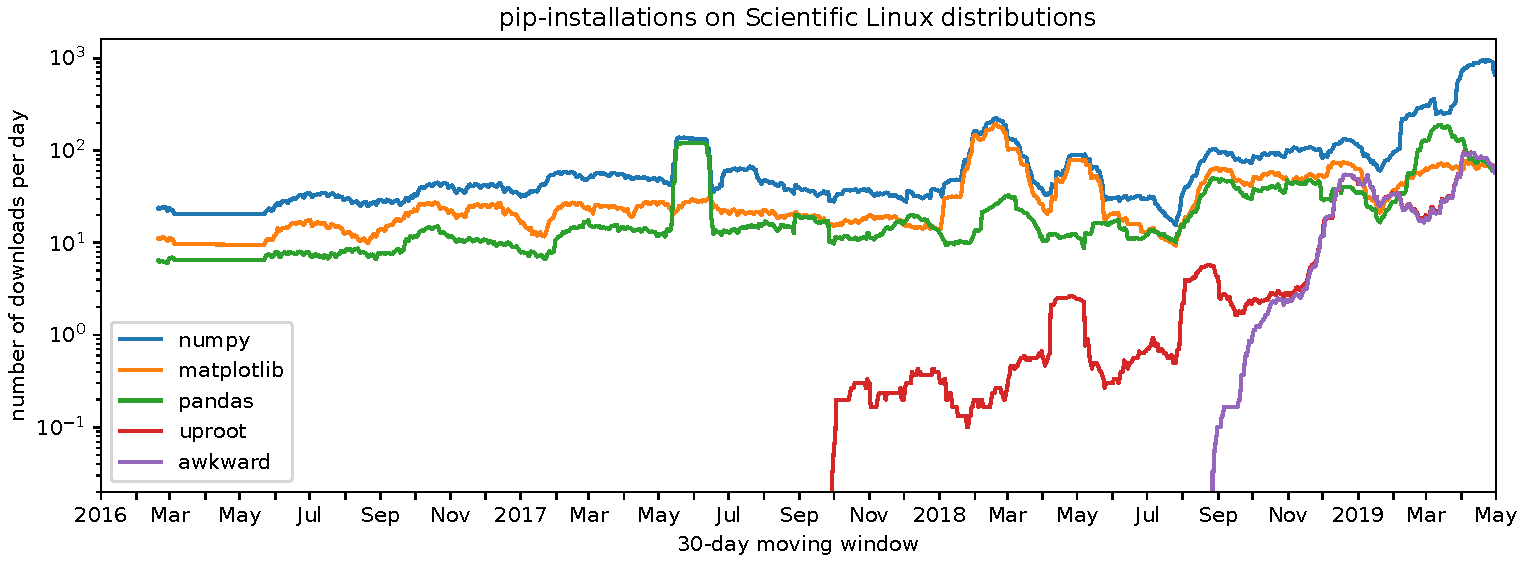
\includegraphics[width=0.9\linewidth]{pip-scientificlinux-uproot.pdf}
\end{center}

\vspace{-0.35 cm}
\begin{itemize}
\item Made a dependency of uproot (reads particle physics data files) last September.

\textcolor{gray}{\normalsize ROOT file $\to$ Numpy or Awkward arrays, depending on structure (majority Awkward).}

\item Hundreds of pip-installations per day; about 1.5 GitHub issues per week.
\item Several user-contributed methods, a dozen more inspired by user needs.
\end{itemize}
\end{columns}
\end{frame}

\begin{frame}{Next steps}
\large
\begin{columns}
\column{0.5\linewidth}
\begin{itemize}
\item At this point, we see some flaws:
\begin{itemize}
\item \mintinline{python}{A.cross(B)} versus \mintinline{python}{awkward.cross(A, B)};
\item should hide \mintinline{python}{JaggedArray}/\mintinline{python}{MaskedArray}/etc.\ structure in a single \mintinline{python}{Array}
\end{itemize}

\item For a long time, we've wanted a versions in C++ (for interfaces) and Numba (to allow procedural programming), but keeping three versions in sync is beyond our resources.

\item So we're rewriting it in four layers (see right).
\end{itemize}

\column{0.5\linewidth}
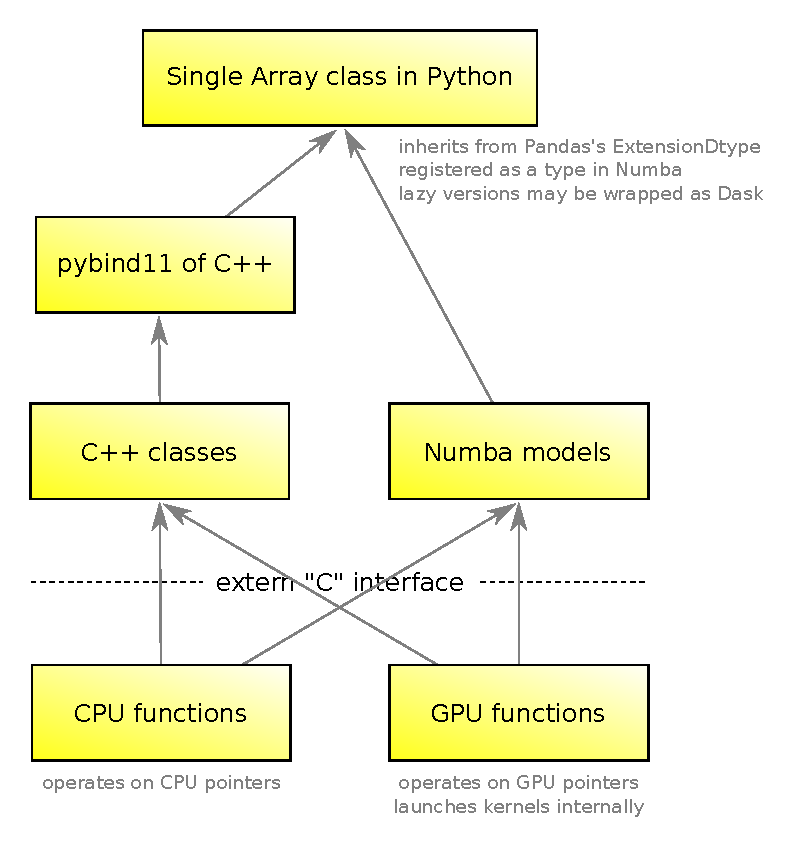
\includegraphics[width=\linewidth]{awkward-1-0-layers.pdf}
\end{columns}
\end{frame}



\begin{frame}{}
\end{frame}

\end{document}
